\documentclass[10pt,a4paper]{article}
\usepackage[utf8]{inputenc}
\usepackage{amsmath}
\usepackage{amsfonts}
\usepackage{graphicx}
\usepackage{amssymb}
\usepackage{bm}
\author{Luc Oth}
\title{Imu Pre-Integration Strategies}

\DeclareMathAlphabet{\mbf}{OT1}{ptm}{b}{n}
\newcommand{\mbs}[1]{{\boldsymbol{#1}}}
\numberwithin{equation}{section}

\begin{document}

\maketitle

\section{Introduction}
The present document describes different integration methods and evaluates their performance with respect to:
\begin{itemize}
\item robustness to integration drift under noisy data
\item robustness of noise propagation under noisy data
\item computational efficiency of the implementation
\end{itemize}

To evaluate the above, we generated random B-spline trajectories on which the accelerometer and gyroscope measurements were sampled. The samples are corrupted with white Gaussian noise.

In the following sections, we will be integrating noisy measurements from an IMU:
\begin{equation}
 _B \tilde { \mbs \omega}_{WB}(t) =  _B \mbs \omega_{WB}(t) + \mbf b^g(t) + \mbs \eta^g(t),
\end{equation}

\begin{equation}
 _B \tilde { \mbs a}_{WB}(t) =  \mbf R_{WB}^T(t)  (_W \mbs a(t) - _W\mbf g )+ \mbf b^a(t) + \mbs \eta^a(t),
\end{equation}

where $_B \tilde{\mbs \omega}_{WB}(t)$ is the rotational velocity observed in the frame of the IMU, $_B \mbf  a_{WB}$ is the acceleration observed in the body frame, $\mbf b$, $\mbf \eta$ are the bias and noise corrupting the measurements. $_W \mbf  g$ is the gravity vector. For readability reasons, we will rely on the sloppy notation $\mbs \omega(t) \leftarrow _B \tilde { \mbs \omega}_{WB}(t)$ and $\mbf a(t) \leftarrow _B \tilde { \mbs a}_{WB}(t)$. Please take note, that a proper integration method operates on the bias and gravity corrected measurements.
We will be sampling the measurements at a fixed or dynamic sampling time referred to as $\Delta t$.

As the standard theory of $\mathcal{R}_3$ applies for the integration of the position and velocity given the measured acceleration, we will focus on the integration theory of the rotational components which has to preserve the structure of the manifold $\mathfrak{so}3$.

In order to propagate the noise, we rely on the covariance of the measurements which is typically given as a covariance matrix of a continuous-time process e.g. $\mbs \Sigma^g$ and the associated $\mbs \eta^g(t)$. In order to apply a noise propagation in discrete time, the continuous-time specification has to be transferred to its discrete-time equivalent:
\begin{equation}
\mbs \Sigma^{gd} = \dfrac{1}{\Delta t} \mbs \Sigma^g,
\end{equation}
with the associated discrete time random process: $\mbs \eta^{gd}_i$.

\section{On-Manifold}

\subsection{Preliminaries}
We will use an intuitive derivation of the integration of rotational velocities on $\mathfrak{so}3$.

Given a rotational velocity $_B \mbs \omega_{WB}$, the associated rotation can be expressed (approximately for small values of $\Delta t$) as:
\begin{equation}
\delta \mbf R(t, \Delta t) = Exp \left( \int_t^{t + \Delta t} \mbs \omega(\tau) d\tau \right).
\end{equation}
It is well known, that composing two rotations parametrized as rotation matrices, $\mbf R_{AB}$, $\mbf R_{BC}$, is simply:
\begin{equation}
\mbf R_{AC} = \mbf R_{AB}\mbf R_{BC},
\end{equation}
where the multiplication is a plain matrix product.
An integration method that preserves the properties of $\mathfrak{so}3$ can thus be defined as infinitesimal compositions of:
\begin{equation}
\mbf R_{WB}(t + \Delta t) = \mbf R_{WB}(t) \delta \mbf R(t, \Delta t).
\label{eq:so3_integration}
\end{equation}

\subsection{Angular Velocity Integration}

\paragraph{Forward Integration}
We take the concepts of equation \eqref{eq:first_order_forward} applied to \eqref{eq:so3_integration}.
The increment $\delta \mbf R$ at time $t_i$ becomes:
\begin{equation}
\delta \mbf R(t_i) = Exp \left( \Delta t \mbs \omega_i\right).
\label{eq:manifold_forward}
\end{equation}

\paragraph{Midward Integration}
With the concepts of equation \eqref{eq:first_order_midward} instead of \eqref{eq:first_order_forward} we obtain the midward integration on the $\mathfrak{so}3$:
\begin{equation}
\delta \mbf R(t_i) = Exp \left( \dfrac{1}{2}\Delta t (\mbs \omega_i + \mbs \omega_{i+1})\right).
\label{eq:manifold_midward}
\end{equation}

\subsection{Noise propagation}
The propagation of the noise $\delta \mbs \phi_{ij}$ (from measurement $j$ to measurement $i$) for the forward on-manifold integration is derived in \cite{forster}. It is only an approximation as a series of linearization steps are taken in the derivations:
\begin{equation}
\delta \mbs \phi_{ij} \approx \Delta \tilde{\mbf R}_{j-1j}^T\delta \mbs \phi_{ij-1} + \mbf J_{r}^{j-1} \mbs \eta_{j-1}^{gd}\Delta t.
\label{eq:manifold_backward}
\end{equation}

$\Delta \tilde{\mbf R}_{j-1j}$ is the change in rotation since the previous integration step (e.g. $\delta \mbf R$ in \eqref{eq:manifold_forward}), $\mbf J_{r}^{j-1}$ is the right-Jacobian of the exponential map from $\mathfrak{so}3$ onto $SO3$.

Although the derivations in \cite{forster} base on a forward integration principle, it is straightforward to show that the results remain valid for a midward integration method using \eqref{eq:manifold_midward}.

Please note, that the Jacobian $\mbf J_{r}^{j-1} \approx \mbf I_3$ for $\delta \mbf R \approx \mbf I_3$ resp. $\Delta t \mbs \omega\approx \mbf 0_3$. As we assume an integration at a rather high frequency, this computationally expensive step can easily be left out. In the evaluations we did not see any difference between the two approaches.

\section{Quaternion}

The derivations below are for Hamiltonian Quaternions (right handed with $\mbf q = \left[ q_w , \textbf{q} \right]$, passive).
Local perturbations appear on the right hand side: $\tilde{\textbf{q}} = \textbf{q}\oplus \Delta \textbf{q}$.
The same convention is used in \cite{joan_sola} where most of the below derivations are available in detail.

\subsection{Preliminaries}

\subsubsection{Time-Derivative of Quaternions (Local)}
\begin{equation}
\dot{\mbf{q}} = \dfrac{1}{2} \mbf{q} \otimes
\begin{bmatrix}
0 \\ \mbs{\omega}
\end{bmatrix}
\end{equation}
with $\mbs{\omega}$ an infinitesimal perturbation (e.g. angular rates). Defining an $\mbs \Omega(\mbs \omega)$, specific to the Hamiltonian quaternion representation:
\begin{equation}
\bm{\Omega}(\mbs{\omega}) = \begin{bmatrix}
0 & -\mbs{\omega}^T \\ \mbs{\omega} & -\left[ \mbs{\omega} \right]_{\times}
\end{bmatrix},
\end{equation}
we get:
\begin{equation}
\dot{\mbf{q}} = \dfrac{1}{2}\mbs{\Omega}(\mbs{\omega}){\mbf{q}}
= \dfrac{1}{2} \mbf{q} \otimes \mbs{\omega},
\label{eq:quaternion_time_derivative}
\end{equation}
and it follows that
\begin{equation}
\dot{\mbf{R}} = \mbf{R}\left[ \mbs{\omega} \right]_\times.
\end{equation}

In the following, $\mbf q \lbrace \cdot \rbrace$ is used to refer to a function that converts a rotation vector representation ($\mbf v = \phi \mbf u$) to a quaternion. One way to achieve this is to use the exponential map $\mbf q = \exp \left( \dfrac{\mbf v}{2} \right)$.


\subsection{Angular Velocity Integration}
An robust and easy way to derive an integration method for quaternions is to use the time-derivative in \eqref{eq:quaternion_time_derivative} and develop the Taylor-series expansion for $\mbf q_{i+1}$:
\begin{equation}
\mbf q_{i+1} = \mbf q_i + \dot{\mbf q}_i \Delta t + \dfrac{1}{2} \ddot{\mbf q}_i \Delta t^2 + \mathcal{O}(\dddot{\mbs q}).
\label{eq:quaternion_taylor_series}
\end{equation}

\subsubsection{Zeroth Order}
Assume that $\mbs \omega = \dot{\mbf q}$ is piece-wise constant (all higher order derivatives are $\mbf 0$), a well trained eye will be able to identify the Taylor series expansion of the exponential map in $\mbs \omega \Delta t$. Thus, follow the below zeroth order integration methods.

\paragraph{Forward}
\begin{equation}
\mbf{q}_{i+1} = \mbf{q}_i \oplus \mbf{q}\lbrace \mbs{\omega}_i \Delta t \rbrace
\end{equation}

\paragraph{Backward}
\begin{equation}
\mbf{q}_{i+1} = \mbf{q}_i \oplus \mbf q \lbrace \mbs{\omega}_{i+1} \Delta t \rbrace
\end{equation}

\paragraph{Midward}
\begin{equation}
\mbf{q}_{i+1} = \mbf{q}_i \oplus \mbf{q}\lbrace \dfrac{\mbs{\omega}_{i+1} + \mbs{\omega}_{i}}{2} \Delta t \rbrace
\end{equation}

All zeroth order quaternion integration methods respect the structure of the quaternion manifold as it is a simple composition of a quaternion with another, infinitesimal, quaternion.

\subsubsection{First Order}

We assume $\mbs \omega = \dot{\mbf q}$ to be piece-wise linear, thus $\ddot{\mbf q}$ constant.
Furthermore we can easily calculate the derivative of $\mbs \omega$: $\dot{\mbs \omega} = \ddot{\mbf q} = \dfrac{\mbs \omega_{i+1} - \mbs \omega_i}{\Delta t}$. 
With some math and again using the Taylor series expansion \eqref{eq:quaternion_taylor_series}:
\begin{equation}
\textbf{q}_{n + 1} \approx \textbf{q}_n \oplus \textbf{q}\lbrace \bar{\bm{\omega}} \Delta t \rbrace
+ \dfrac{\Delta t^2}{24} \textbf{q}_n \oplus \begin{bmatrix}
0 \\ \bm \omega_n \times \bm \omega_{n+1}
\end{bmatrix}
\end{equation}
where the first term is equivalent to the zeroth order midwards integration.

According to \cite{joan_sola} the order of magnitude of the second term is around $10^{-6} ||\bm \omega ||$ and often smaller.
While the zeroth order integration methods preserve the structure of the quaternion manifold, the sum in the first order integration does not.
The norm of the resulting quaternion should be checked regularly and re-normalized if required.

\subsubsection{Runge-Kutta}
Section \ref{sec:runge-kutta} shows the Runge-Kutta method to integrate a generic function $\dot{\mbf x} = f(\mbf x, t)$, which in the case of quaternions becomes:
\begin{equation}
\dot{\mbf q} = f(\mbf q(t), \mbs \omega(t)) = \dfrac{1}{2} \mbf q \oplus \mbs \omega = \dfrac{1}{2} \mbs \Omega(\mbs \omega) {\mbf q}.
\end{equation}

In the case of a Hamiltonian parametrization of the quaternion,
\begin{equation}
\mbs \Omega(\mbs \omega) = \begin{bmatrix}
0 & -w_0 & -w_1 & -w_2 \\
w_0 & 0 & w_2 & -w1 \\
w_1 & -w_2 & 0 & w_0 \\
w_2 & w_1 & -w_0 & 0
\end{bmatrix}
\end{equation}

It is expected that both measurements $\mbs \omega_i$ and $\mbs \omega_{i+1}$ are available. A $\tilde{\cdot}$ is used to refer to temporary values of $\mbf q$.

\paragraph{Third Order}
Applying the Runge-Kutta algorithm to our measurement model with quaternions results in
\begin{align*}
\mbf k_1 &= \mbs \omega_i &
\dot{\mbf q}_1 &= f({\mbf q}_i , \mbf k_1) &
\tilde{\mbf q}_1 &= \mbf q_i +\dfrac{1}{2} \Delta t \dot{\mbf q}_1 \\
\mbf k_2 &= \mbs \omega_i + \dfrac{1}{2}\left( \mbs \omega_{i+1} - \mbs \omega_i \right) &
\dot{\mbf q}_2 &= f(\tilde{\mbf q}_1 , \mbf k_2) &
\tilde{\mbf q}_2 &= \mbf q_i + \Delta t \left(-\dot{\mbf q}_1 + 2 \dot{\mbf q}_2 \right) \\
\mbf k_3  &=  \mbs \omega_{i+1} &
\dot{\mbf q}_3 &= f(\tilde{\mbf q}_2 , \mbf k_3). &
\end{align*}
The above notation is not entirely consistent with section \ref{sec:runge-kutta}, where $\mbf k$ is what is here called $\dot{\mbf q}$, and $\mbf k$ represents an intermediate step to approximate the rotational velocity in between $\mbs w_i$ and $\mbs w_{i+1}$.

The final result is obtained by combining all intermediate results:
\begin{equation}
\mbf q_{i+1} = \mbf q_i + \dfrac{1}{6} \Delta t \left(
	\dot{\mbf q}_1 +
	4 \dot{\mbf q}_2 +
	\dot{\mbf q}_3
\right).
\label{eq:rk3}
\end{equation}

\paragraph{Fourth Order}
Similar to the third order case, we apply the Runge-Kutta algorithm up to fourth order:
\begin{align*}
\mbf k_1 &= \mbs \omega_i &
\dot{\mbf q}_1 &= f({\mbf q}_i , \mbf k_1) &
\tilde{\mbf q}_1 &= \mbf q_i +\dfrac{1}{2} \Delta t \dot{\mbf q}_1 \\
\mbf k_2 &= \mbs \omega_i + \dfrac{1}{2}\left( \mbs \omega_{i+1} - \mbs \omega_i \right) &
\dot{\mbf q}_2 &= f(\tilde{\mbf q}_1, \mbf k_2) &
\tilde{\mbf q}_2 &= \mbf q_i +\dfrac{1}{2} \Delta t \dot{\mbf q}_2 \\
\mbf k_3 &= \mbs \omega_i + \dfrac{1}{2}\left( \mbs \omega_{i+1} - \mbs \omega_i \right) &
\dot{\mbf q}_3 &= f(\tilde{\mbf q}_2, \mbf k_3) &
\tilde{\mbf q}_2 &= \mbf q_i + \Delta t \dot{\mbf q}_3 \\
\mbf k_4  &=  \mbs \omega_{i+1} &
\dot{\mbf q}_4 &= f(\tilde{\mbf q}_3 , \mbf k_4), &
\end{align*}

and finally
\begin{equation}
\mbf q_{i+1} = \mbf q_i + \dfrac{1}{6} \Delta t \left(
	\dot{\mbf q}_1 +
	2 \dot{\mbf q}_2 +
	2 \dot{\mbf q}_3 +
	\dot{\mbf q}_4
\right).
\label{eq:rk4}
\end{equation}

Neither the linear interpolation of the quaternion derivatives, nor the summations preserve the quaternion manifold - although they are valid approximations for small values. To obtain valid results, $\mbf q_{i+1}$ has to be re-normalized in every step.

\subsubsection{Crouch-Grossman}

A major drawback of a Runge-Kutta integration is that it is designed for values that evolve in $\mathcal{R}_4$.
Quaternions, however, only evolve on a subspace of $\mathcal{R}_4$, namely the unit sphere.
The Crouch-Grossman Lie Group method defines the Runge-Kutta method directly on the $\mathfrak{so}3$ manifold.
A basic introduction is available in \cite{andrle_crassidist} and the thorough derivations in \cite{crouch_grossman}.
The generalized formulas for arbitrary orders are also available in the literature, we restrict ourselves to the third and fourth order.

\paragraph{Third Order}

\begin{align*}
\mbf k_1 & = \mbs \omega_i \\
\mbf k_2 & = \mbs \omega_i + \dfrac{3}{4} \left( \mbs \omega_{i+1} - \mbs \omega_i \right) \\
\mbf k_2 & = \mbs \omega_i + \dfrac{17}{24} \left( \mbs \omega_{i+1} - \mbs \omega_i \right)
\end{align*}

\begin{equation}
	\mbf q_{i+1} = \mbf q_i 
	\exp \left( \dfrac{13}{51} \Delta t \mbf k_1 \right)
	\exp \left( -\dfrac{2}{3} \Delta t \mbf k_2 \right)
	\exp \left( \dfrac{24}{17} \Delta t \mbf k_3 \right).
\end{equation}

\paragraph{Fourth Order}
The fourth order method requires a total of five steps. The determination of the coefficients it not trivial and only numerical values are available.

\begin{align*}
\mbf k_1 & = \mbs \omega_i \\
\mbf k_2 & = \mbs \omega_i + c_2 \left( \mbs \omega_{i+1} - \mbs \omega_i \right) \\
\mbf k_2 & = \mbs \omega_i + c_3 \left( \mbs \omega_{i+1} - \mbs \omega_i \right) \\
\mbf k_2 & = \mbs \omega_i + c_4 \left( \mbs \omega_{i+1} - \mbs \omega_i \right) \\
\mbf k_2 & = \mbs \omega_i + c_5 \left( \mbs \omega_{i+1} - \mbs \omega_i \right)
\end{align*}

\begin{equation}
	\mbf q_{i+1} = \mbf q_i 
	\exp \left(b_1 \Delta t \mbf k_1 \right)
	\exp \left(b_2 \Delta t \mbf k_2 \right)
	\exp \left(b_3 \Delta t \mbf k_3 \right)
	\exp \left(b_4 \Delta t \mbf k_4 \right)
	\exp \left(b_5 \Delta t \mbf k_5 \right).
\end{equation}

With the coefficients $b_i$ and $c_i$  as below:

\begin{align*}
b_1 &= 0.1370831520630755 & c_1 & = 0 \\
b_2 & = -0.0183698531564020 & c_2 & = 0.8177227988124852 \\
b_3 & =0.7397813985370780 & c_3 & = 0.3859740639032449 \\
b_4 & = -0.1907142565505889 & c_4 & = 0.3242290522866937 \\
b_5 & = 0.3322195591068374 & c_5 & = 0.8768903263420429.
\end{align*}

\subsection{Noise Propagation}
As we did not observe any significant differences between our implementations of noise propagation, we restrict our evaluations to the zeroth order, and third and fourth order Runge-Kutta methods. 

Define a rotational error state, $\delta \mbs \theta$, such that $\delta \mbf R \approx \mbf I_3 + \left[ \delta \mbs \theta \right]_\times$ resp. $\delta \mbs \theta \approx \begin{bmatrix}
1 & \delta \mbs \theta / 2
\end{bmatrix}^T$. We also define a function $\mbf R \lbrace \cdot \rbrace$ that, similar to $\mbf q \lbrace \cdot \rbrace$, converts its arbitrary argument to a rotation matrix.

The noise covariance, $\mbf Q_{\mbf \eta}$, is propagated under a Gaussian noise assumption in a linear system following a basic Kalman Filter principle:
\begin{equation}
\mbs \Sigma_{i+1} = \mbf A \mbs \Sigma_i \mbf A^T + \mbf Q_{\mbf \eta},
\end{equation}
$\mbf A$ describes how small changes of the state $\mbf x$ are propagated. For a linear system it takes the form 
\begin{equation}
\mbf x_{i+1} = \mbf A \mbf x_i.
\label{eq:discrete_state_propagation}
\end{equation}
The noise covariance $\mbf Q_{\mbf \eta}$ is the integrated discrete-time sensor noise during the time interval $\Delta t$:
\begin{equation}
\mbf Q_{\mbf \eta} = \mbs \Sigma^d \Delta t^2 = \mbs \Sigma \Delta t.
\label{eq:integrated_noise_covariance}
\end{equation}

\subsubsection{Zeroth Order}
Following the derivations in \cite{joan_sola}, one will come up with the (simplified) error state dynamics in the form of \eqref{eq:discrete_state_propagation}
\begin{equation}
\delta \mbs \theta_{i+1} = \mbf R^T \lbrace \mbs \omega \Delta t \rbrace
\delta  \mbs \theta_i + \mbs \theta_I,
\end{equation}
$\mbs \theta_I$ being the initial value (typically $\mbf 0$).

The covariance of the rotational error state is finally propagated using:
\begin{equation}
\mbs \Sigma_{i+1}^{\delta \mbs \theta} = \mbf R^T \lbrace \mbs \omega_i \Delta t \rbrace
\mbs \Sigma_{i}^{\delta \mbs \theta}
\mbf R \lbrace \mbs \omega_i \Delta t \rbrace + 
\mbs \Sigma^{\mbs \omega}_i \Delta t
\label{eq:covariance_first_order}
\end{equation}

Equation \eqref{eq:covariance_first_order}, shown for a forward integration, is independent of the applied zeroth order integration type. The equivalent midward variant is obtained by replacing $\mbs \omega_i$ with the corresponding midward value $\dfrac{1}{2} (\mbs \omega_{i+1} + \mbs \omega_i)$.

\subsubsection{Runge-Kutta}
Given a linear continuous-time state system
\begin{equation}
\dot{\mbf x} = \mbf A(t) \mbf x(t),
\end{equation}
one can define a discrete-time state transition matrix $\mbs \Phi_{t_{i+1} | t_i}$ that describes the change of the state $\mbf x_i$ from time step $t_{i}$ to $t_{i+1}$
\begin{equation}
\mbf x(t_{i+1}) = \mbs \Phi_{t_{i+1} | t_i} \mbf x(t_i).
\end{equation}
Please note, that  $\mbs \Phi_{t_{i} | t_i} = \mbf I$.
The transition matrix is directly used to propagate the noise covariance between discrete time-steps:
\begin{equation}
\mbs \Sigma_{i+1}^{\delta \mbs \theta} = \mbs \Phi_{t_{i+1} | t_i}
\mbs \Sigma_{i}^{\delta \mbs \theta}
\mbs \Phi_{t_{i+1} | t_i}^T
 + 
\mbs \Sigma^{\mbs \omega}_i \Delta t.
\label{eq:covariance_rk}
\end{equation}

With the Runge-Kutta approach directly applied to the dynamic state transition matrix we obtain the corresponding discrete state transition matrix.

\paragraph{Third Order}

Given the intermediate states $\tilde{\mbf q}_{\lbrace 1,2,3 \rbrace}$ and $\mbf k_{\lbrace 1, 2, 3 \rbrace}$ from \eqref{eq:rk3}

\begin{align*}
\mbs \Phi_0 & = \mbf I_3 & \\
\dot{\mbs \Phi}_1 & = \left[\mbf k_1 \right]_\times \mbs \Phi_0 &
	\mbs \Phi_1 & = \mbs \Phi_0 + \dfrac{1}{2} \Delta t \dot{\mbs \Phi}_1 \\
\dot{\mbs \Phi}_2 & = \left[\mbf k_2 \right]_\times \mbs \Phi_1 &
	\mbs \Phi_2 & = \mbs \Phi_0 + \Delta t \left( - \dot{\mbs \Phi}_1 + 2 \dot{\mbs \Phi}_2  \right) \\
\dot{\mbs \Phi}_3 & = \left[\mbf k_3 \right]_\times \mbs \Phi_2
\end{align*}

\begin{equation}
\mbs \Phi_{i+1} = \mbf I_3 + \dfrac{1}{6} \Delta t \left(
	\dot{\mbs \Phi}_1 + 4 \dot{\mbs \Phi}_2 + \dot{\mbs \Phi}_3
\right).
\end{equation}


\paragraph{Fourth Order}

Given the intermediate states $\tilde{\mbf q}_{\lbrace 1, 2, 3, 4 \rbrace}$ and $\mbf k_{\lbrace 1, 2, 3, 4 \rbrace}$ from \eqref{eq:rk4}

\begin{align*}
\mbs \Phi_0 & = \mbf I_3 & \\
\dot{\mbs \Phi}_1 & = \left[\mbf k_1 \right]_\times \mbs \Phi_0 &
	\mbs \Phi_1 & = \mbs \Phi_0 + \dfrac{1}{2} \Delta t \dot{\mbs \Phi}_1 \\
\dot{\mbs \Phi}_2 & = \left[\mbf k_2 \right]_\times \mbs \Phi_1 &
	\mbs \Phi_2 & = \mbs \Phi_0 + \dfrac{1}{2} \Delta t \dot{\mbs \Phi}_2 \\
\dot{\mbs \Phi}_3 & = \left[\mbf k_3 \right]_\times \mbs \Phi_2 &
	\mbs \Phi_3 & = \mbs \Phi_0 + \Delta t \dot{\mbs \Phi}_3  \\
\dot{\mbs \Phi}_4 & = \left[\mbf k_4 \right]_\times \mbs \Phi_3
\end{align*}

\begin{equation}
\mbs \Phi_{i+1} = \mbf I_3 + \dfrac{1}{6} \Delta t \left(
	\dot{\mbs \Phi}_1 + 2 \dot{\mbs \Phi}_2 + 2 \dot{\mbs \Phi}_3 + \dot{\mbs \Phi}_4
\right).
\end{equation}


\section{Results}

\subsection{Setup}

The data used in the experiments in this section was generated using a continuous-time parametrization of a randomly generated trajectory.
The trajectory is parametrized as a $n$'th order, 6-dimensional B-Spline where: i) the first three elements represent a translation; ii) the last three elements a rotation-vector parametrization of a rotation.
We are fully aware of the limitations of a rotation vector parametrization but given the known setup, the use is safe.

The order of the B-Spline was chosen to be at least $n = 5$ to ensure non-constant accelerations but varied during the experiments.
The number of basis functions was set to at least $50$, and the regularization weight used for the initialization of the spline was set to max. $0.0001$.
The order, number of basis functions and regularization weight was varied during the experiments to obtain  trajectories of different complexity levels.
Details on modelling 3-dimensional motion as a continous-time B-Spline are best looked up in \cite{furgale}.

The simulated rotational velocity measurements are perturbed with white Gaussian noise with noise density $\sigma = 0.000186$, corresponding to one of our real calibrations.

The parameters of the rotation-vector parametrization of a sample curve used for evaluation is given in Figure \ref{fig:sample_rotation_curve} and \ref{fig:sample_rotation_curve_aggressive}.

To save space in the graphics and result tables, the integrations will be referred to by numbers. Table \ref{tbl:method_number} shows the mapping of index to integration method.

\begin{table}
\begin{center}
\begin{tabular}{ l | l }
0  & Manifold Forward \\
1  & Manifold Midward \\
2  & Quaternion Forward \\
3  & Quaternion Midward \\
4  & Quaternion Runge-Kutta 3 \\
5  & Quaternion Runge-Kutta 4 \\
6  & Quaternion Crouch-Grossmann 3\\
7  & Quaternion Crouch-Grossmann 4
\end{tabular}
\end{center}
\caption{Implemented integration methods and corresponding number.}
\label{tbl:method_number}
\end{table}




\begin{figure}
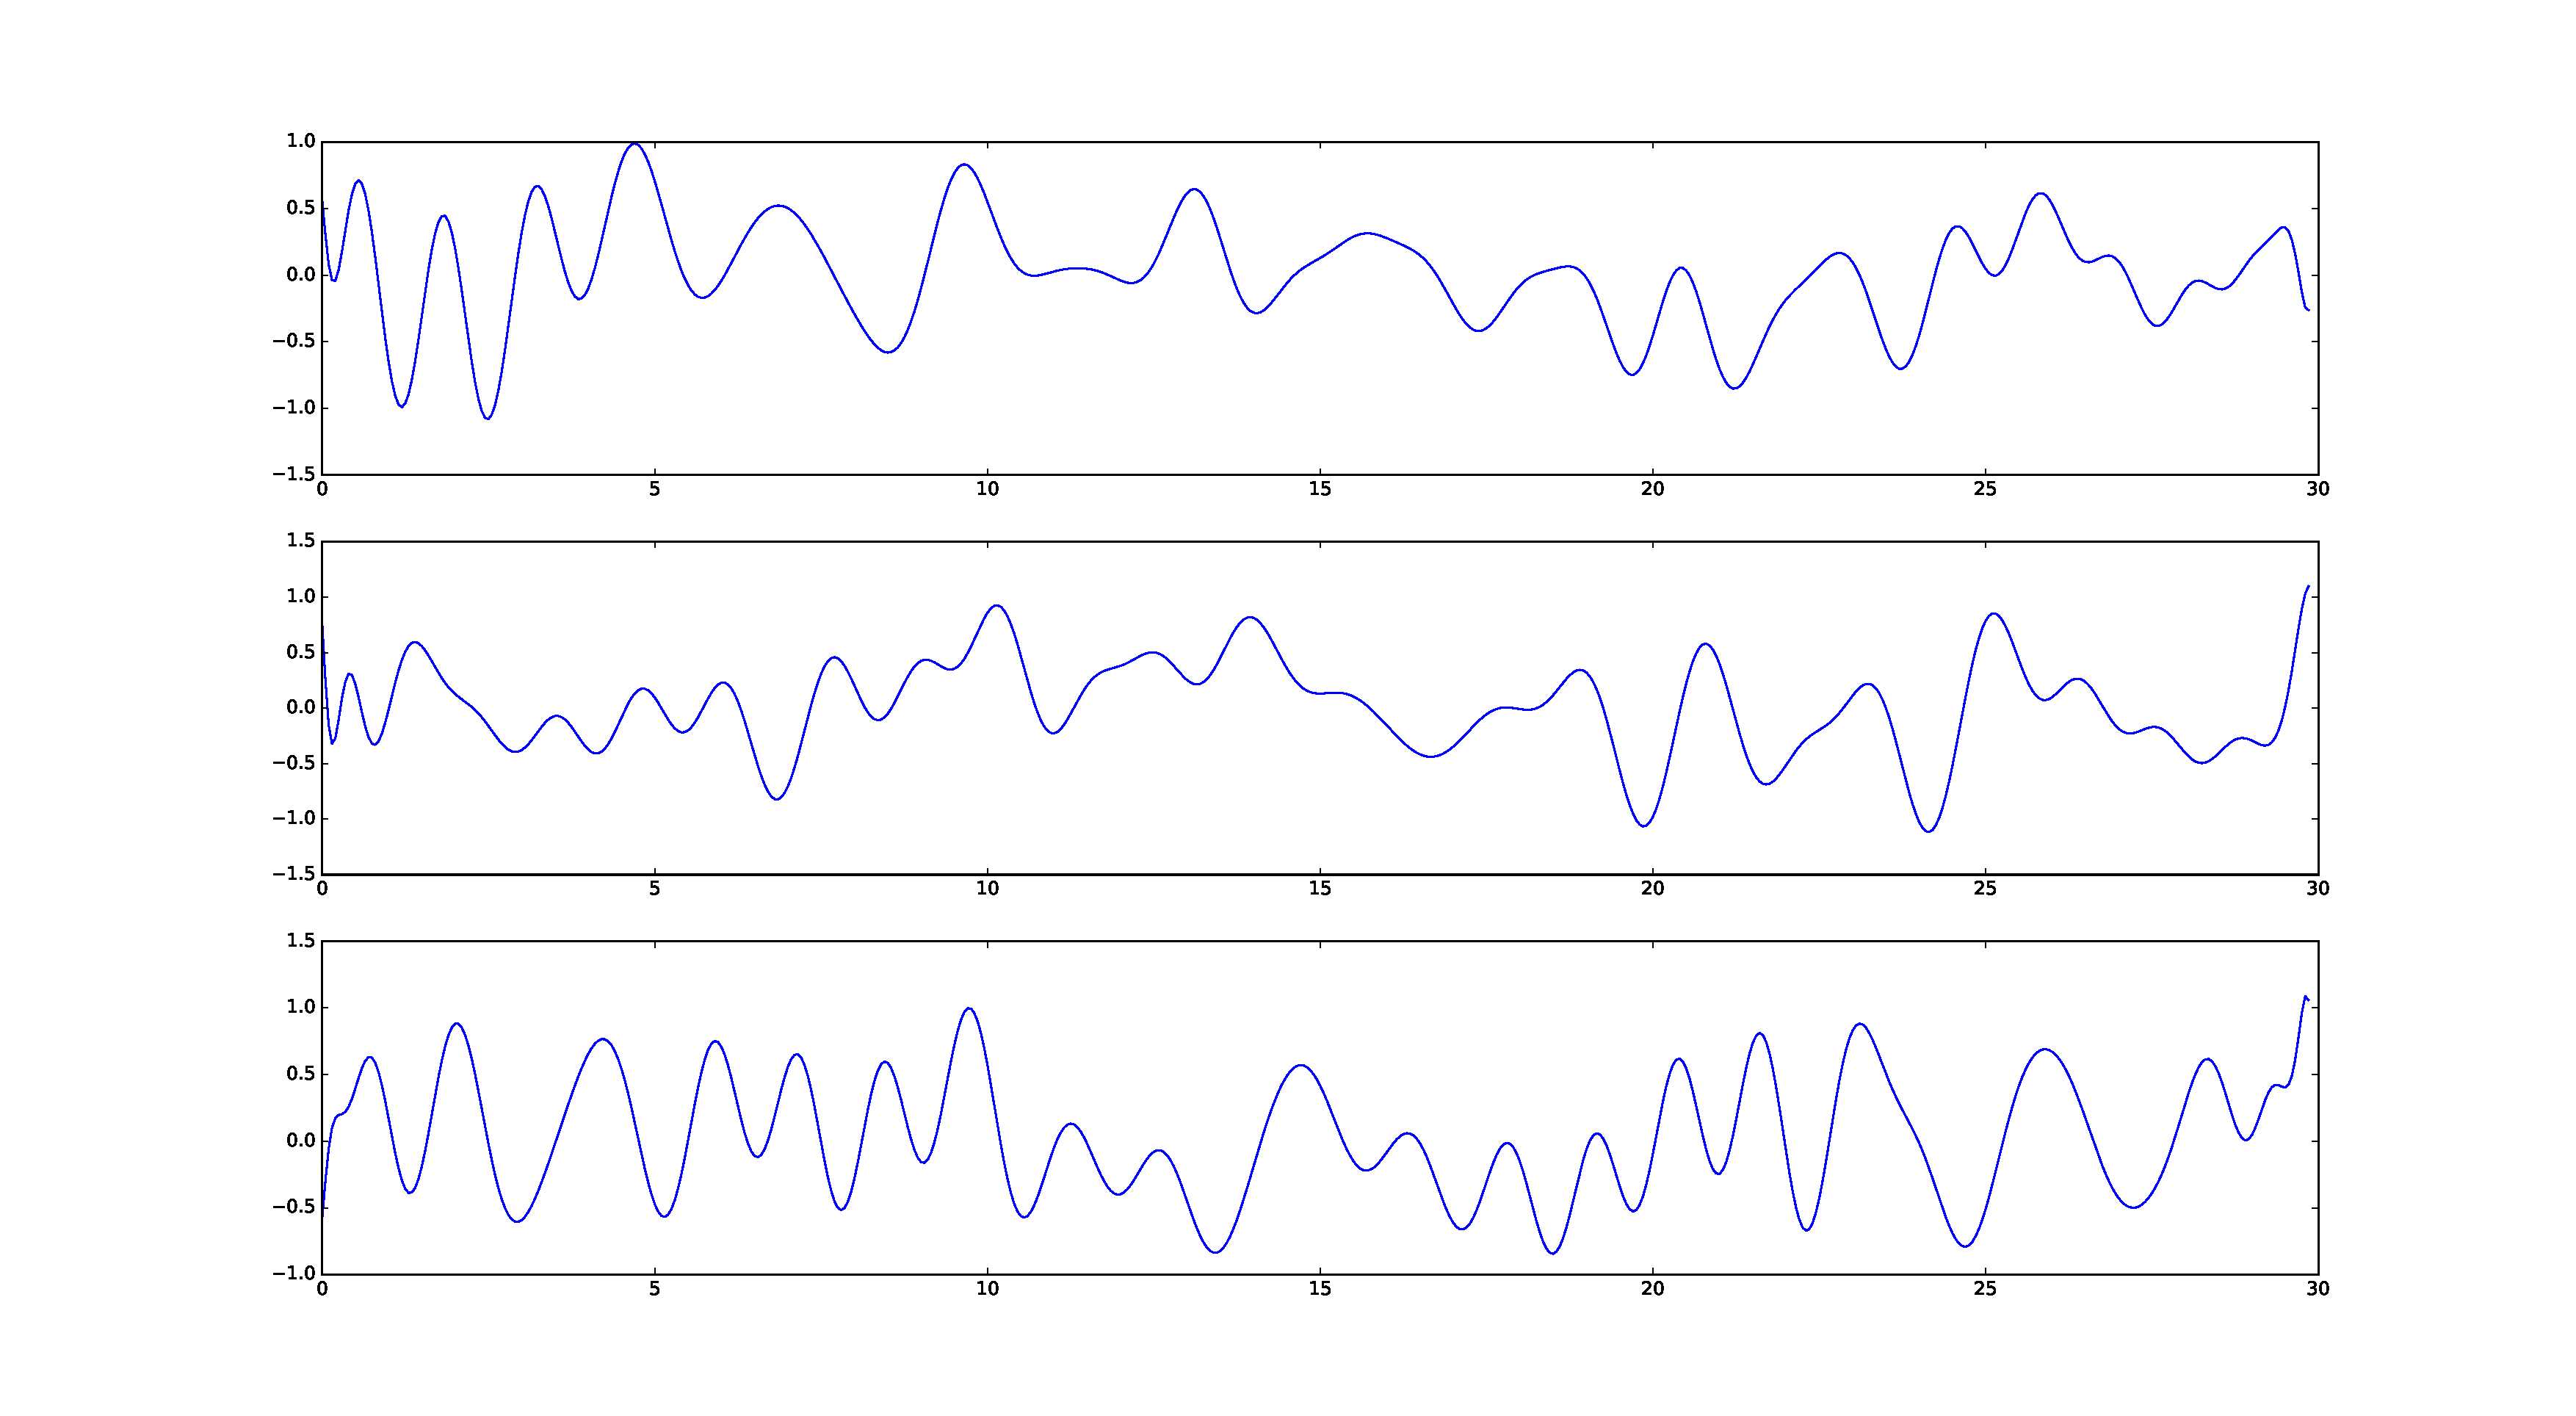
\includegraphics[width=14cm]{figures/sample_rotation_vector_curve.pdf}
\caption{Sample trajectory used to generate the results. The $x$, $y$, $z$ components of the rotation-vector parametrization.}
\label{fig:sample_rotation_curve}
\end{figure}	

\begin{figure}
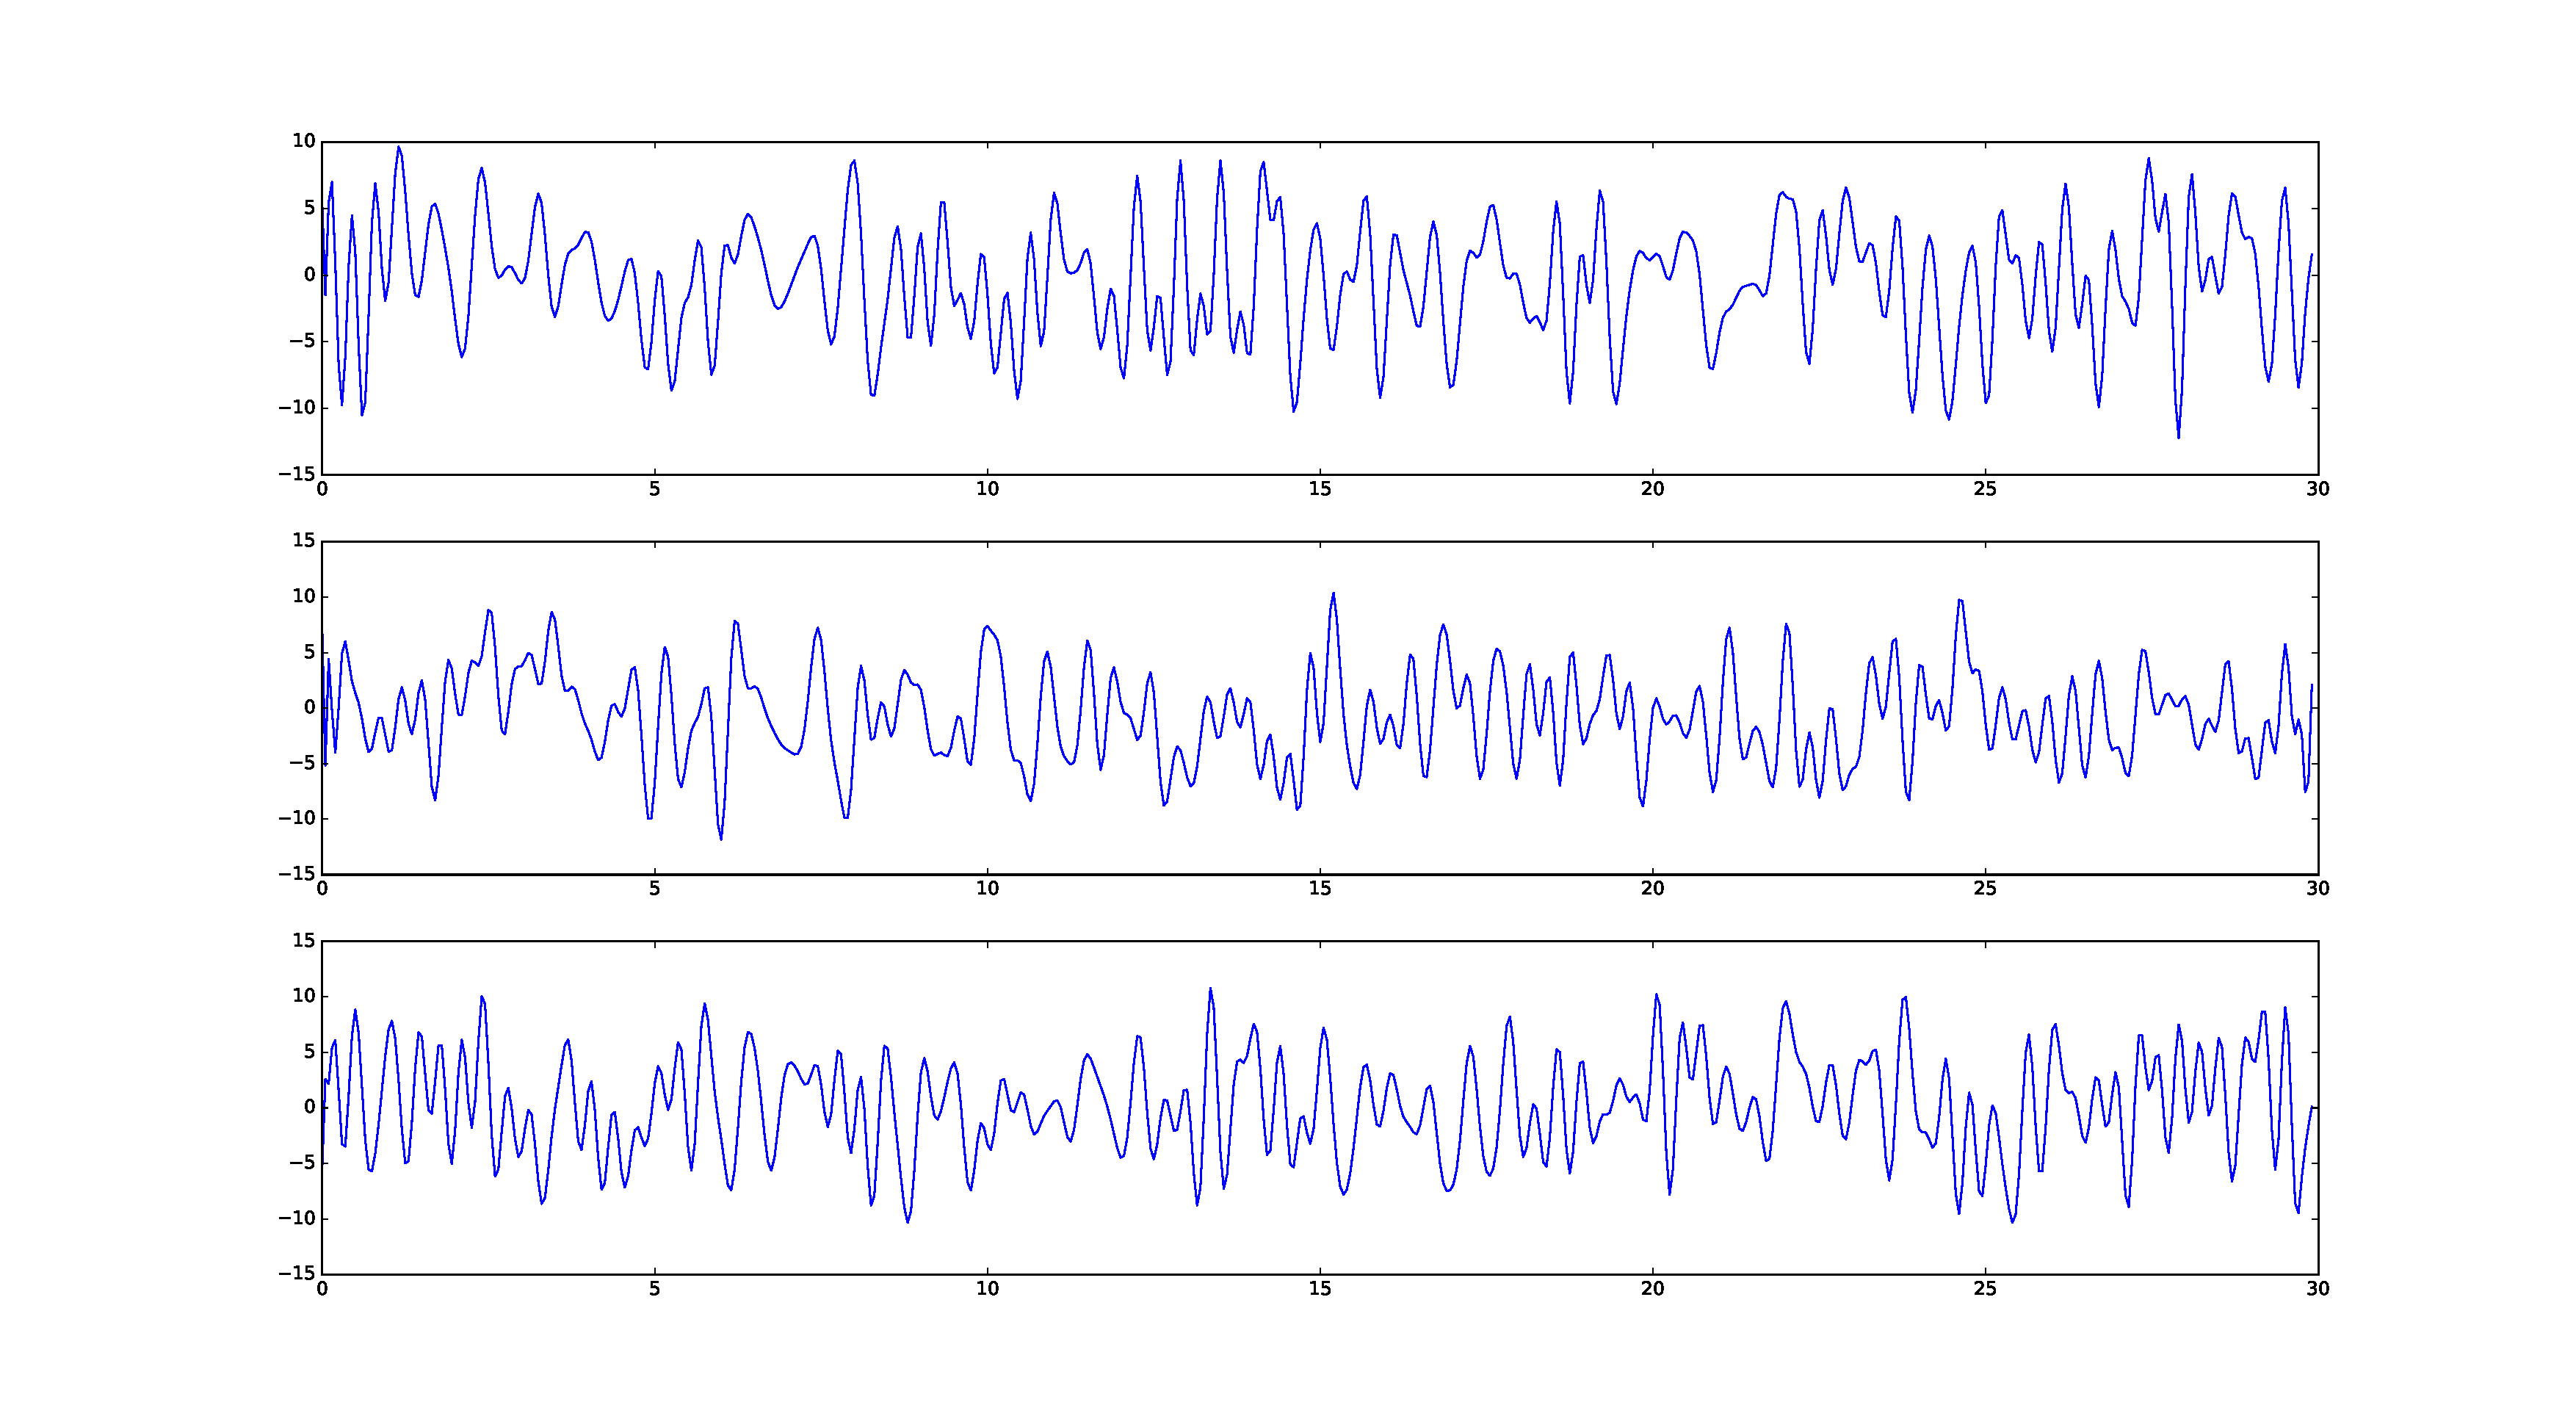
\includegraphics[width=14cm]{figures/sample_rotation_vector_curve_aggressive.pdf}
\caption{Sample trajectory used to generate the results. The $x$, $y$, $z$ components of the rotation-vector parametrization for an aggressive rotational motion ($10 \times$ larger).}
\label{fig:sample_rotation_curve_aggressive}
\end{figure}	

\subsection{Integration Drift under Noise}

\subsubsection{Integration Drift}

We ran all integration methods introduced in the previous section on randomly generated trajectories.
The rotational velocity $\omega$ was corrupted with Gaussian noise.
To obtain statistically relevant results, despite the noisy signals, all $8$ methods were used on $200$ different trajectories with independently sampled Gaussian noise. The generated trajectories are $30$ seconds long.
Figure \ref{fig:rotation_integration_drift_boxplot} shows the resulting cumulative drift errors in a box-plot. The numerical values are available in Table \ref{tbl:rotation_integration_drift}

Both the manifold and quaternion forward methods are clearly inferior to all higher order methods.
The midward integration methods perform an implicit low-pass filtering which reduces the drift by reducing the effect of the uncertainty that a single measurement would introduce.
The higher order methods - $4$'th order Runge-Kutta, and $3$rd and $4$th order Crouch-Grossman - only slightly improve over the midpoint methods.

\begin{figure}
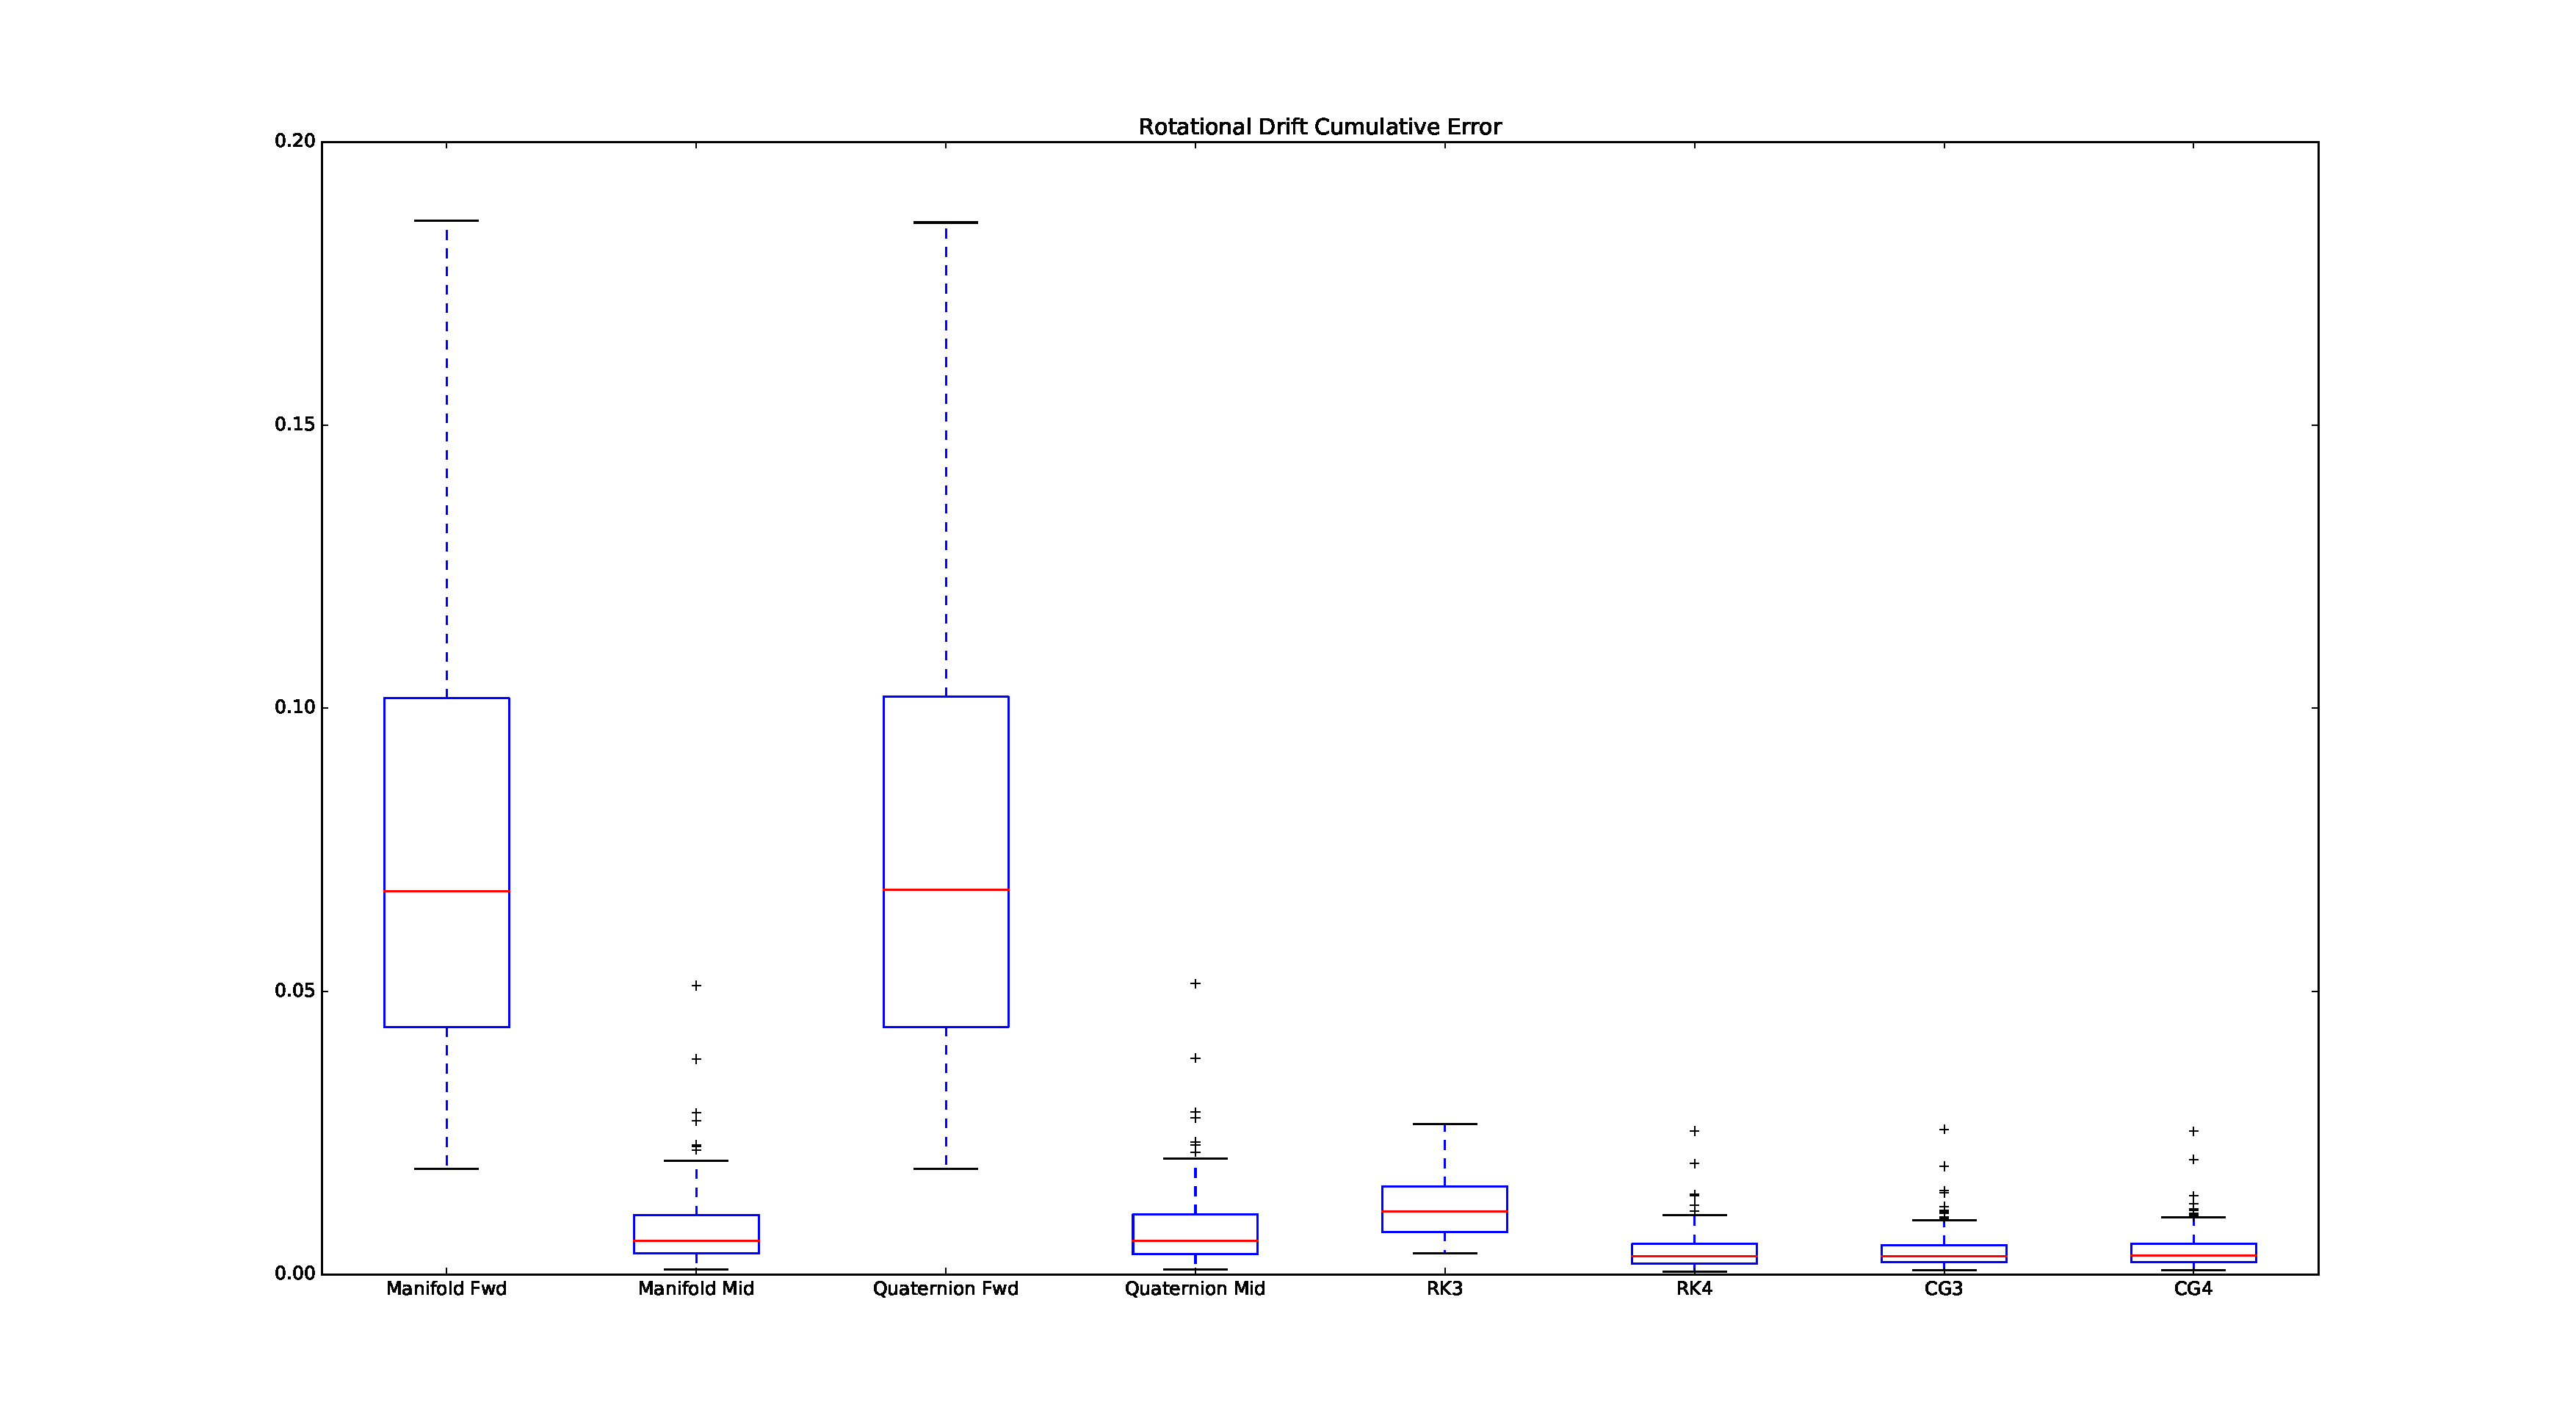
\includegraphics[width=14cm]{figures/rotation_integration_drift_boxplot.pdf}
\caption{}
\label{fig:rotation_integration_drift_boxplot}
\end{figure}	

\begin{table}
\begin{center}
\begin{tabular}{ l | l || l }
0  & Manifold Forward &  0.0749788\\
1  & Manifold Midward &  0.00785299 \\
2  & Quaternion Forward &  0.0750557 \\
3  & Quaternion Midward & 0.00787657\\
4  & Quaternion Runge-Kutta 3 & 0.0120488 \\
5  & Quaternion Runge-Kutta 4 & 0.00411811 \\
6  & Quaternion Crouch-Grossmann 3 & 0.00418711\\
7  & Quaternion Crouch-Grossmann 4 & 0.00419546
\end{tabular}
\end{center}
\caption{Average cumulative drift of different integration methods after $200$ runs on simulated trajectories. Spline-Order: $5$, Noise $\sigma = 0.00186$, rotation multiplier $5$, $50$ segments.}
\label{tbl:rotation_integration_drift}
\end{table}

The integration methods were tested against a set of trajectories of different complexity, for every set, $200$ runs were performed. Table \ref{tbl:rotation_integration_drift_run_parameters} summarizes the parameters used to generate the said trajectories. Figure \ref{fig:average_cumulative_drift} shows the results graphically and the averages are available in Table \ref{tbl:rotation_integration_drift_values}.

\begin{table}
\begin{center}
\begin{tabular}{ l | l | l | l | l | l | l}
Run & $Hz$ & Spline Order & Noise ($1e4$) & Segments & Smoothing & Rotation Multiplier \\
0 & 200 & 5 & 1.86 & 50 & $1e-4$ & 1 \\
1 & 200 & 5 & 3.72 & 50 &  $1e-4$ & 1 \\
2 & 200 & 5 & 7.44 & 50 &  $1e-4$ & 1 \\
3 & 20  & 5 & 1.86 & 50 &  $1e-4$ & 1 \\
4 & 200  & 10 & 1.86 & 50 &  $1e-4$ & 1 \\
5 & 200  & 10 & 1.86 & 200 &  $1e-4$ & 1 \\
6 & 200  & 10 & 1.86 & 200 & $1e-6$ & 1 \\
7 & 200  & 10 & 1.86 & 50 & $1e-4$ & 10 \\
8 & 200  & 10 & 1.86 & 50 & $1e-4$ & 5
\end{tabular}
\end{center}
\caption{Parameters used to generate different trajectories for the drift evaluation.}
\label{tbl:rotation_integration_drift_run_parameters}
\end{table}

\begin{table}
\begin{center}
\begin{tabular}{ l | l | l | l | l | l | l | l | l | l}
 & 0 & 1 & 2 & 3 & 4 & 5 & 6 & 7 & 8 \\
0 & 3.94058 & 3.93493 & 3.94597 & 0.418478 & 2.04392 & 3.174 & 9.72347 & 0.135967 & 7.49788 \\
1 & 0.107683 & 0.200063 & 0.401721 & 4.24869 & 0.116234 & 0.31039 & 1.275 & 2.90529 & 0.785299 \\
2 & 3.94248 & 3.95241 & 3.96111 & 0.418429 & 2.03719 & 3.18374 & 9.72697 & 0.135978 & 7.50557 \\
3 & 0.112839 & 0.1992 & 0.410831 & 4.24528 & 0.117766 & 0.313399 & 1.28355 & 2.90502 & 0.787657 \\
4 & 0.688499 & 0.7136 & 0.768424 & 9.30135 & 0.345993 & 0.587262 & 1.61293 & 2.82292 & 1.20488 \\
5 & 0.109847 & 0.208381 & 0.386993 & 3.26243 & 0.10692 & 0.178501 & 0.860189 & 1.47977 & 0.411811 \\
6 & 0.104299 & 0.200145 & 0.403532 & 3.28245 & 0.107502 & 0.174976 & 0.861394 & 1.47441 & 0.418711 \\
7 & 0.105074 & 0.202421 & 0.398457 & 3.24674 & 0.108499 & 0.179947 & 0.862777 & 1.46404 & 0.419546
\end{tabular}
\end{center}
\caption{Average values for different trajectories. The rows are the different integration methods, the columns show the different trajectories.}
\label{tbl:rotation_integration_drift_values}
\end{table}

\begin{figure}
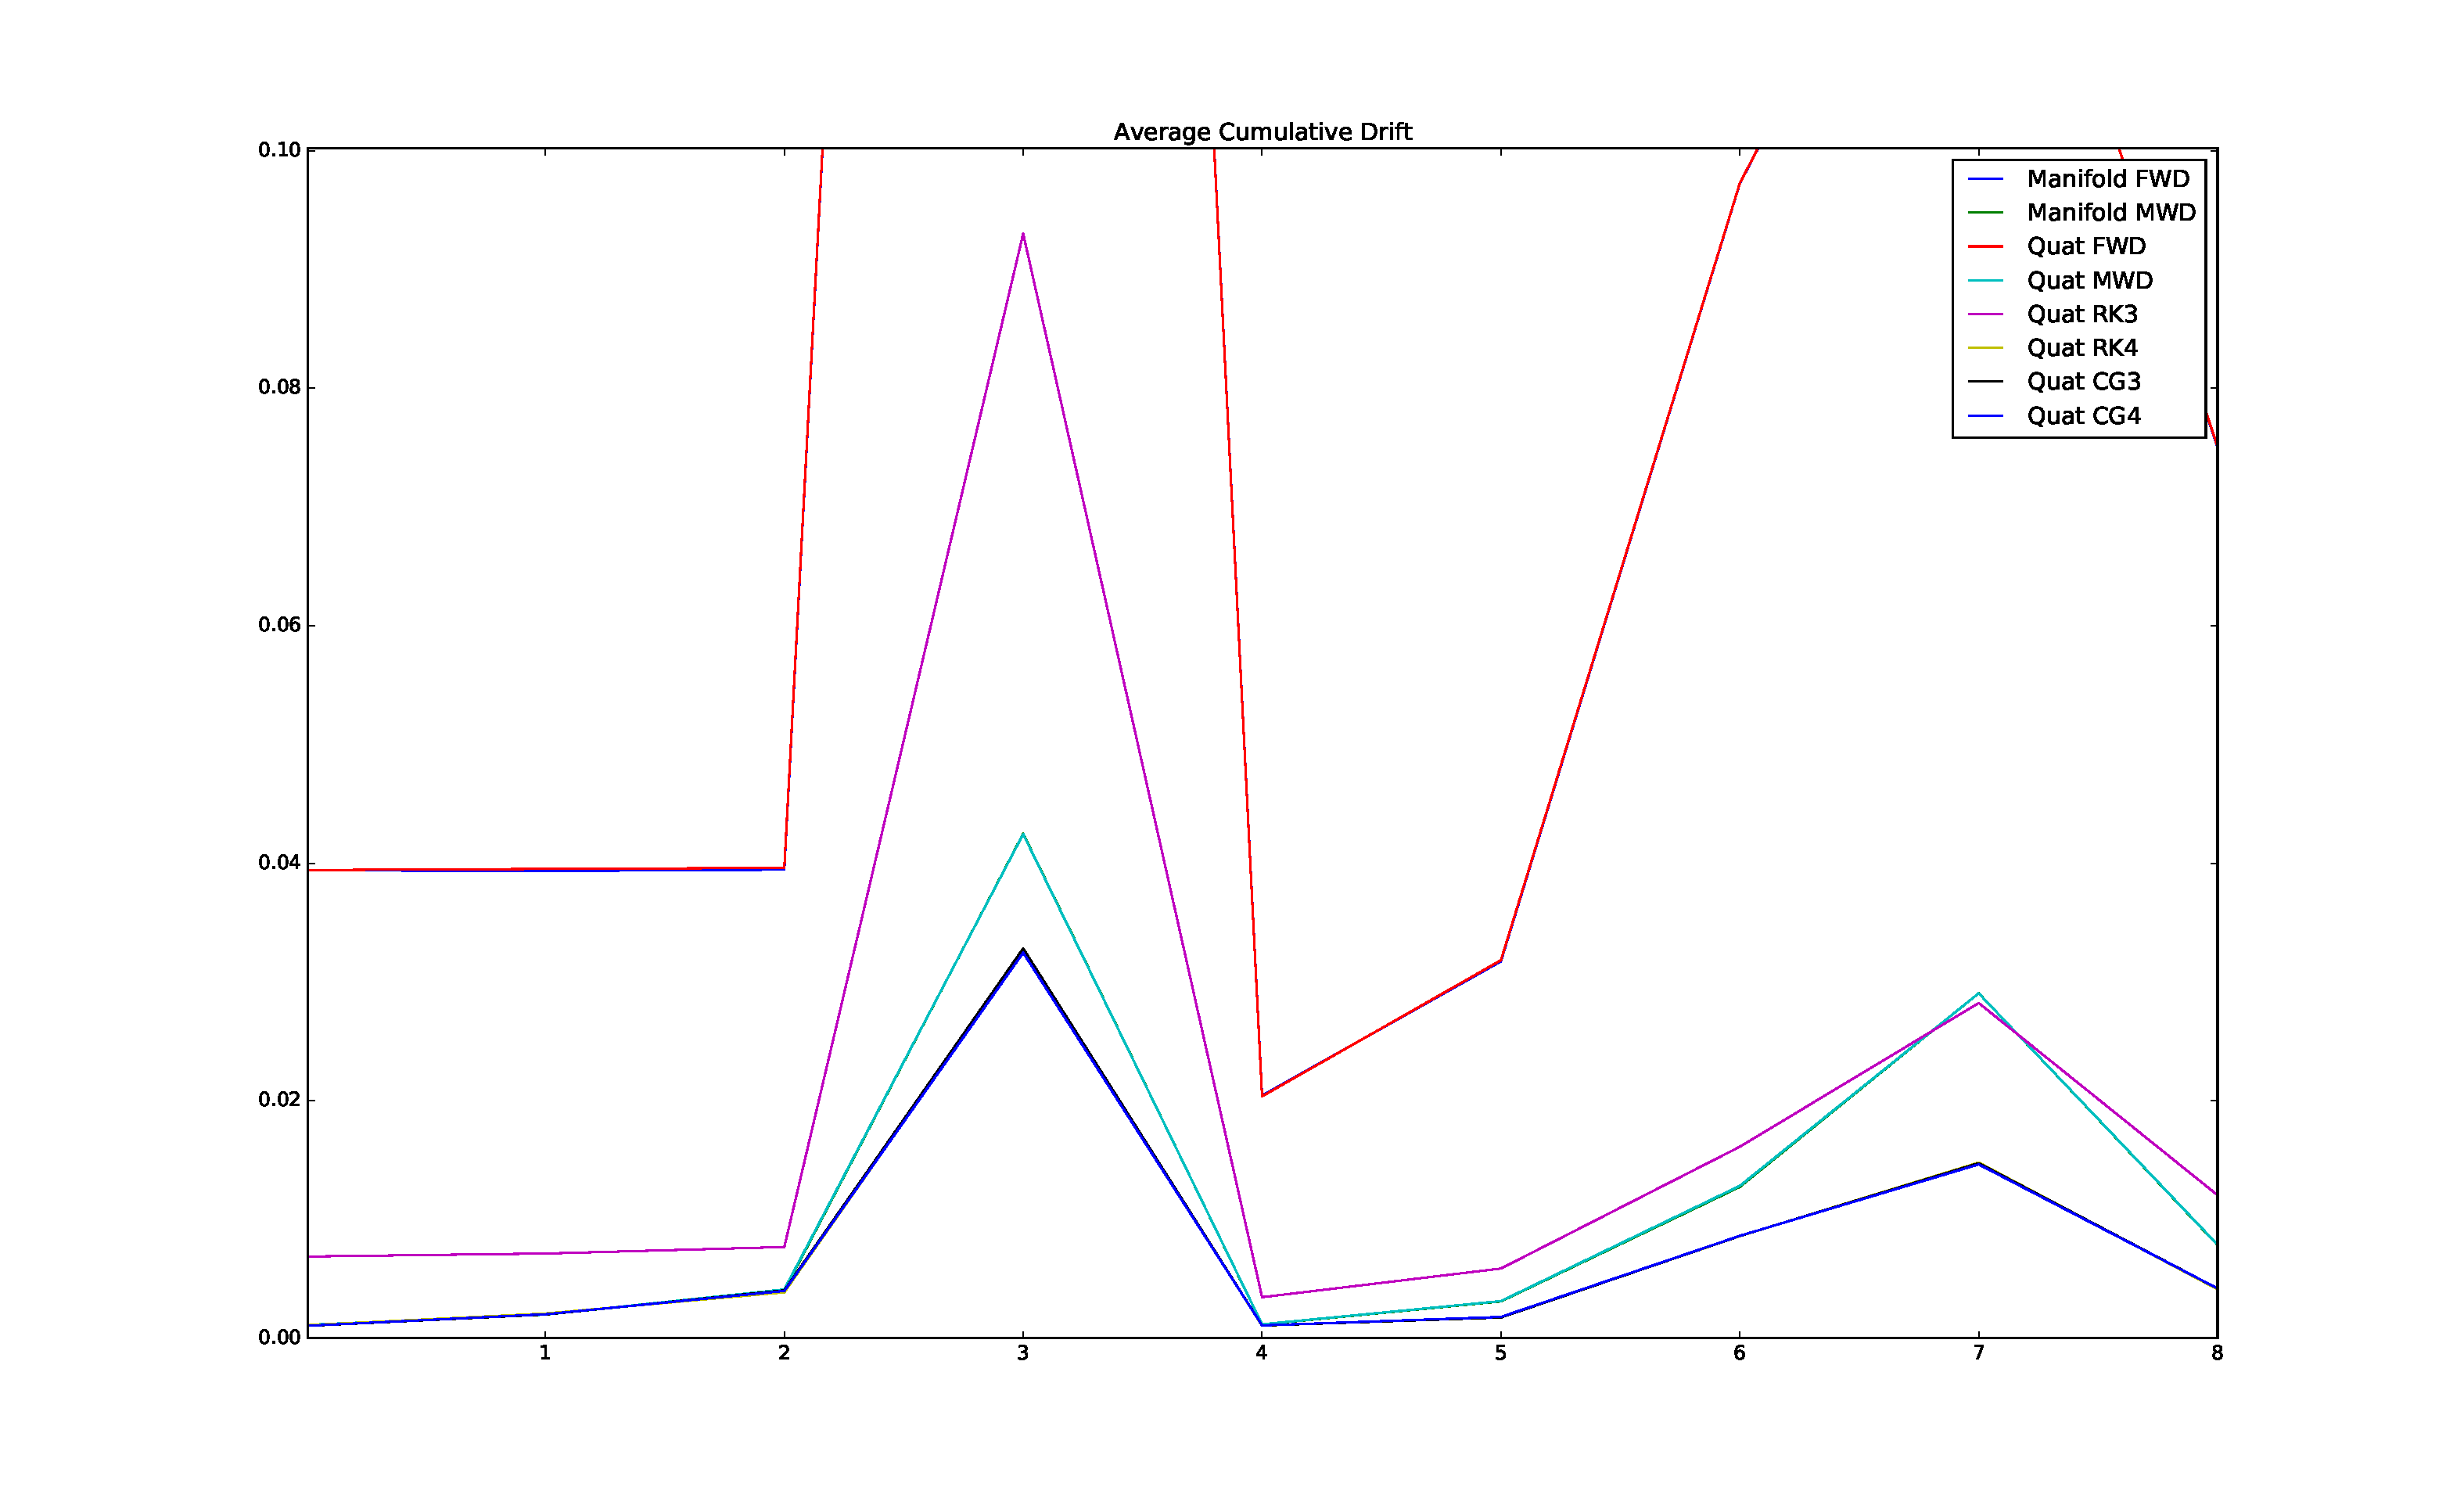
\includegraphics[width=14cm]{figures/average_cumulative_drift.pdf}
\caption{Average cumulative drift for runs with different trajectories}
\label{fig:average_cumulative_drift}
\end{figure}	

\subsubsection{Real Dataset}

The rotation integration was performed on a real dataset of the EUROC series (MH\_01\_easy).
The ground-truth bias was used to correct the gyroscope measurements prior to integration, Figure \ref{fig:rotation_drift_real}.

\begin{figure}
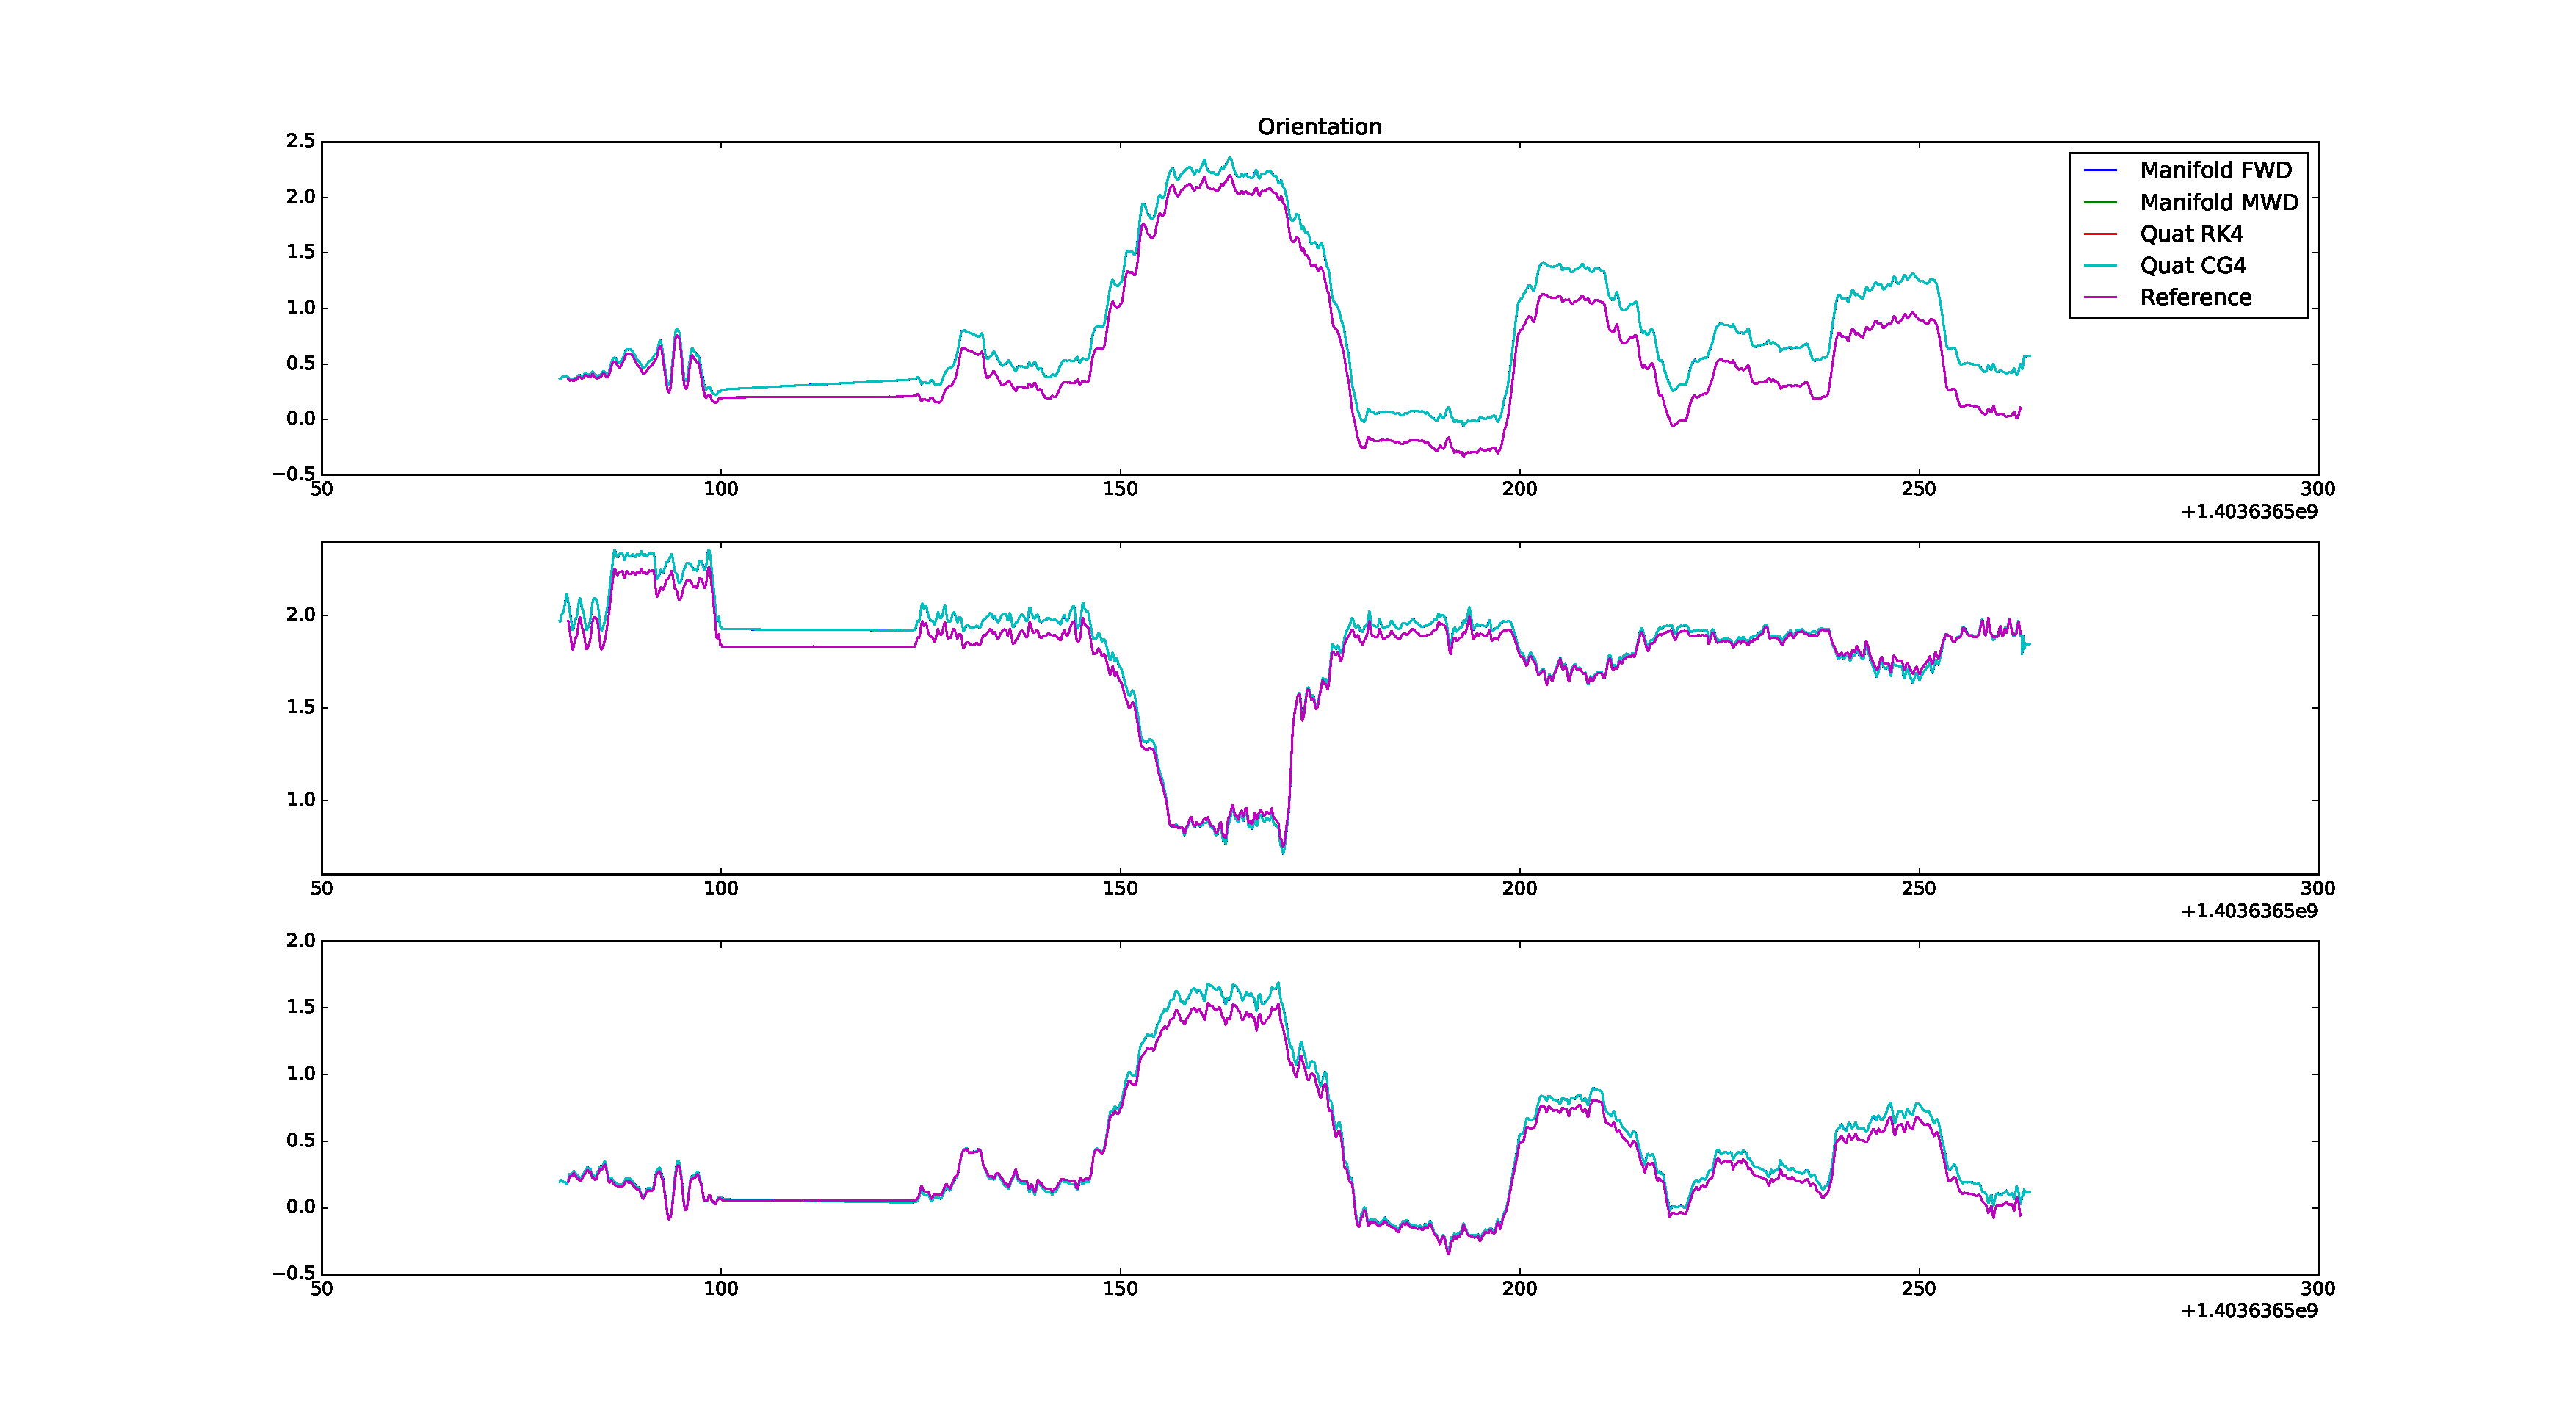
\includegraphics[width=14cm]{figures/rotation_drift_real.pdf}
\caption{Integration drift evaluated on a real dataset where the ground-truth drift was subtracted prior to integration. The plots show the $x$, $y$ and $z$ coordinates of a rotation vector parametrization.}
\label{fig:rotation_drift_real}
\end{figure}	

As a matter of fact, the magnitude of the uncertainty on the bias' Brownian motion, typically of magnitude $1e-4$ or $1e-5$, appears to massively outweigh the drift accountable to the integrator choice, producing cumulative errors in the range of $1e-3$ after integrations of $6000$ measurements over $30$ seconds.
For a measurement stream at above $100$Hz, the choice of integrator appear to be rather irrelevant given the scale of the influencing uncertainties.
However, discarding forward and backward integrators appears to be a good choice performance and complexity-wise.

\subsection{Noise Propagation}
The noise propagation is evaluated based on a Monte-Carlo simulation of the integration and a subsequent variance estimation of the resulting drift. Typically, $20 000$ Monte-Carlo runs were performed.

The covariance at every integration step is estimated by calculating the error state of the integrated value with a ground-truth value:
\begin{equation}
\delta \mbs \theta = \log \left( \delta \mbs R_{ground-truth}^T \delta \mbs R_{estimate} \right),
\end{equation}
$\log$ is the matrix logarithm of a vector on $\mathfrak{se}3$.

The similarity of two covariance matrices is expressed using the matrix norm:
\begin{equation}
\delta \Sigma = || \mbs \Sigma_{ground-truth} - \mbs \Sigma_{estimated} ||
\end{equation}

There are no significant differences between the proposed integration methods. Except for the $3$rd order Runge-Kutta method which seems to become less stable in the presence of fast rotation changes.

\begin{figure}
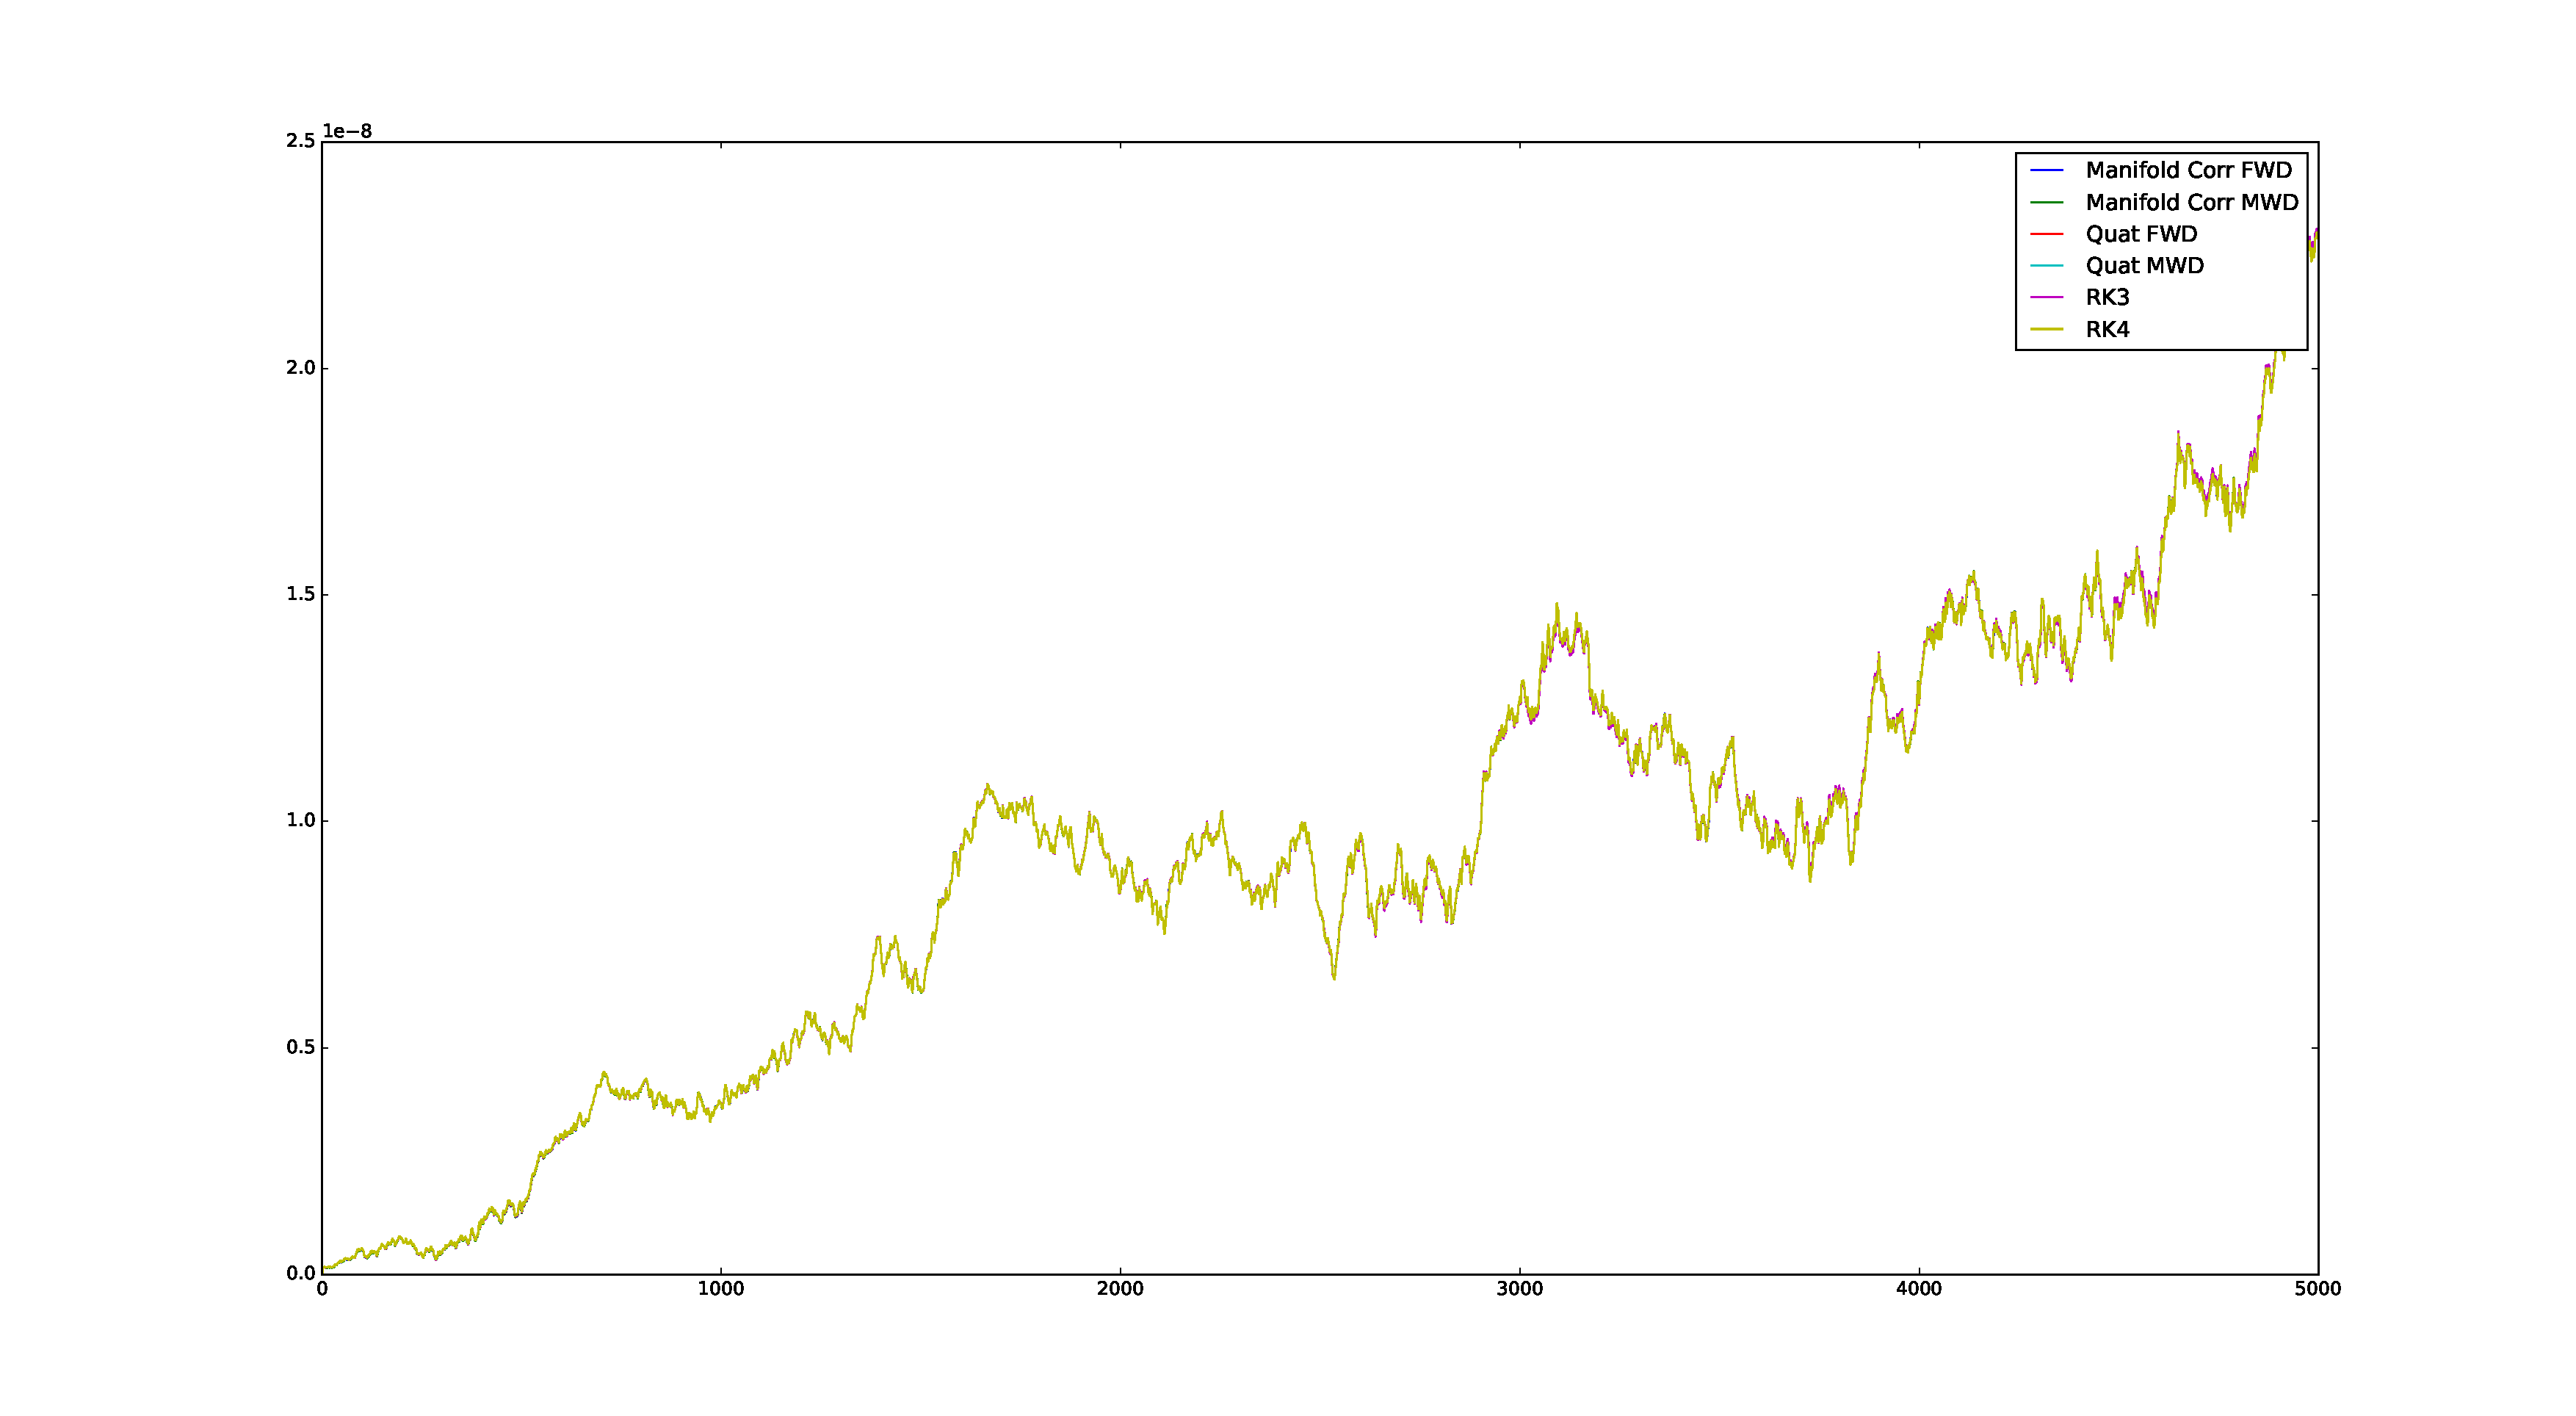
\includegraphics[width=14cm]{figures/covariance_offset.pdf}
\caption{Noise propagation for a noise density of $1.86e-4$, $\Delta t = 0.005$. }
\label{fig:covariance_propagation}
\end{figure}	

\begin{figure}
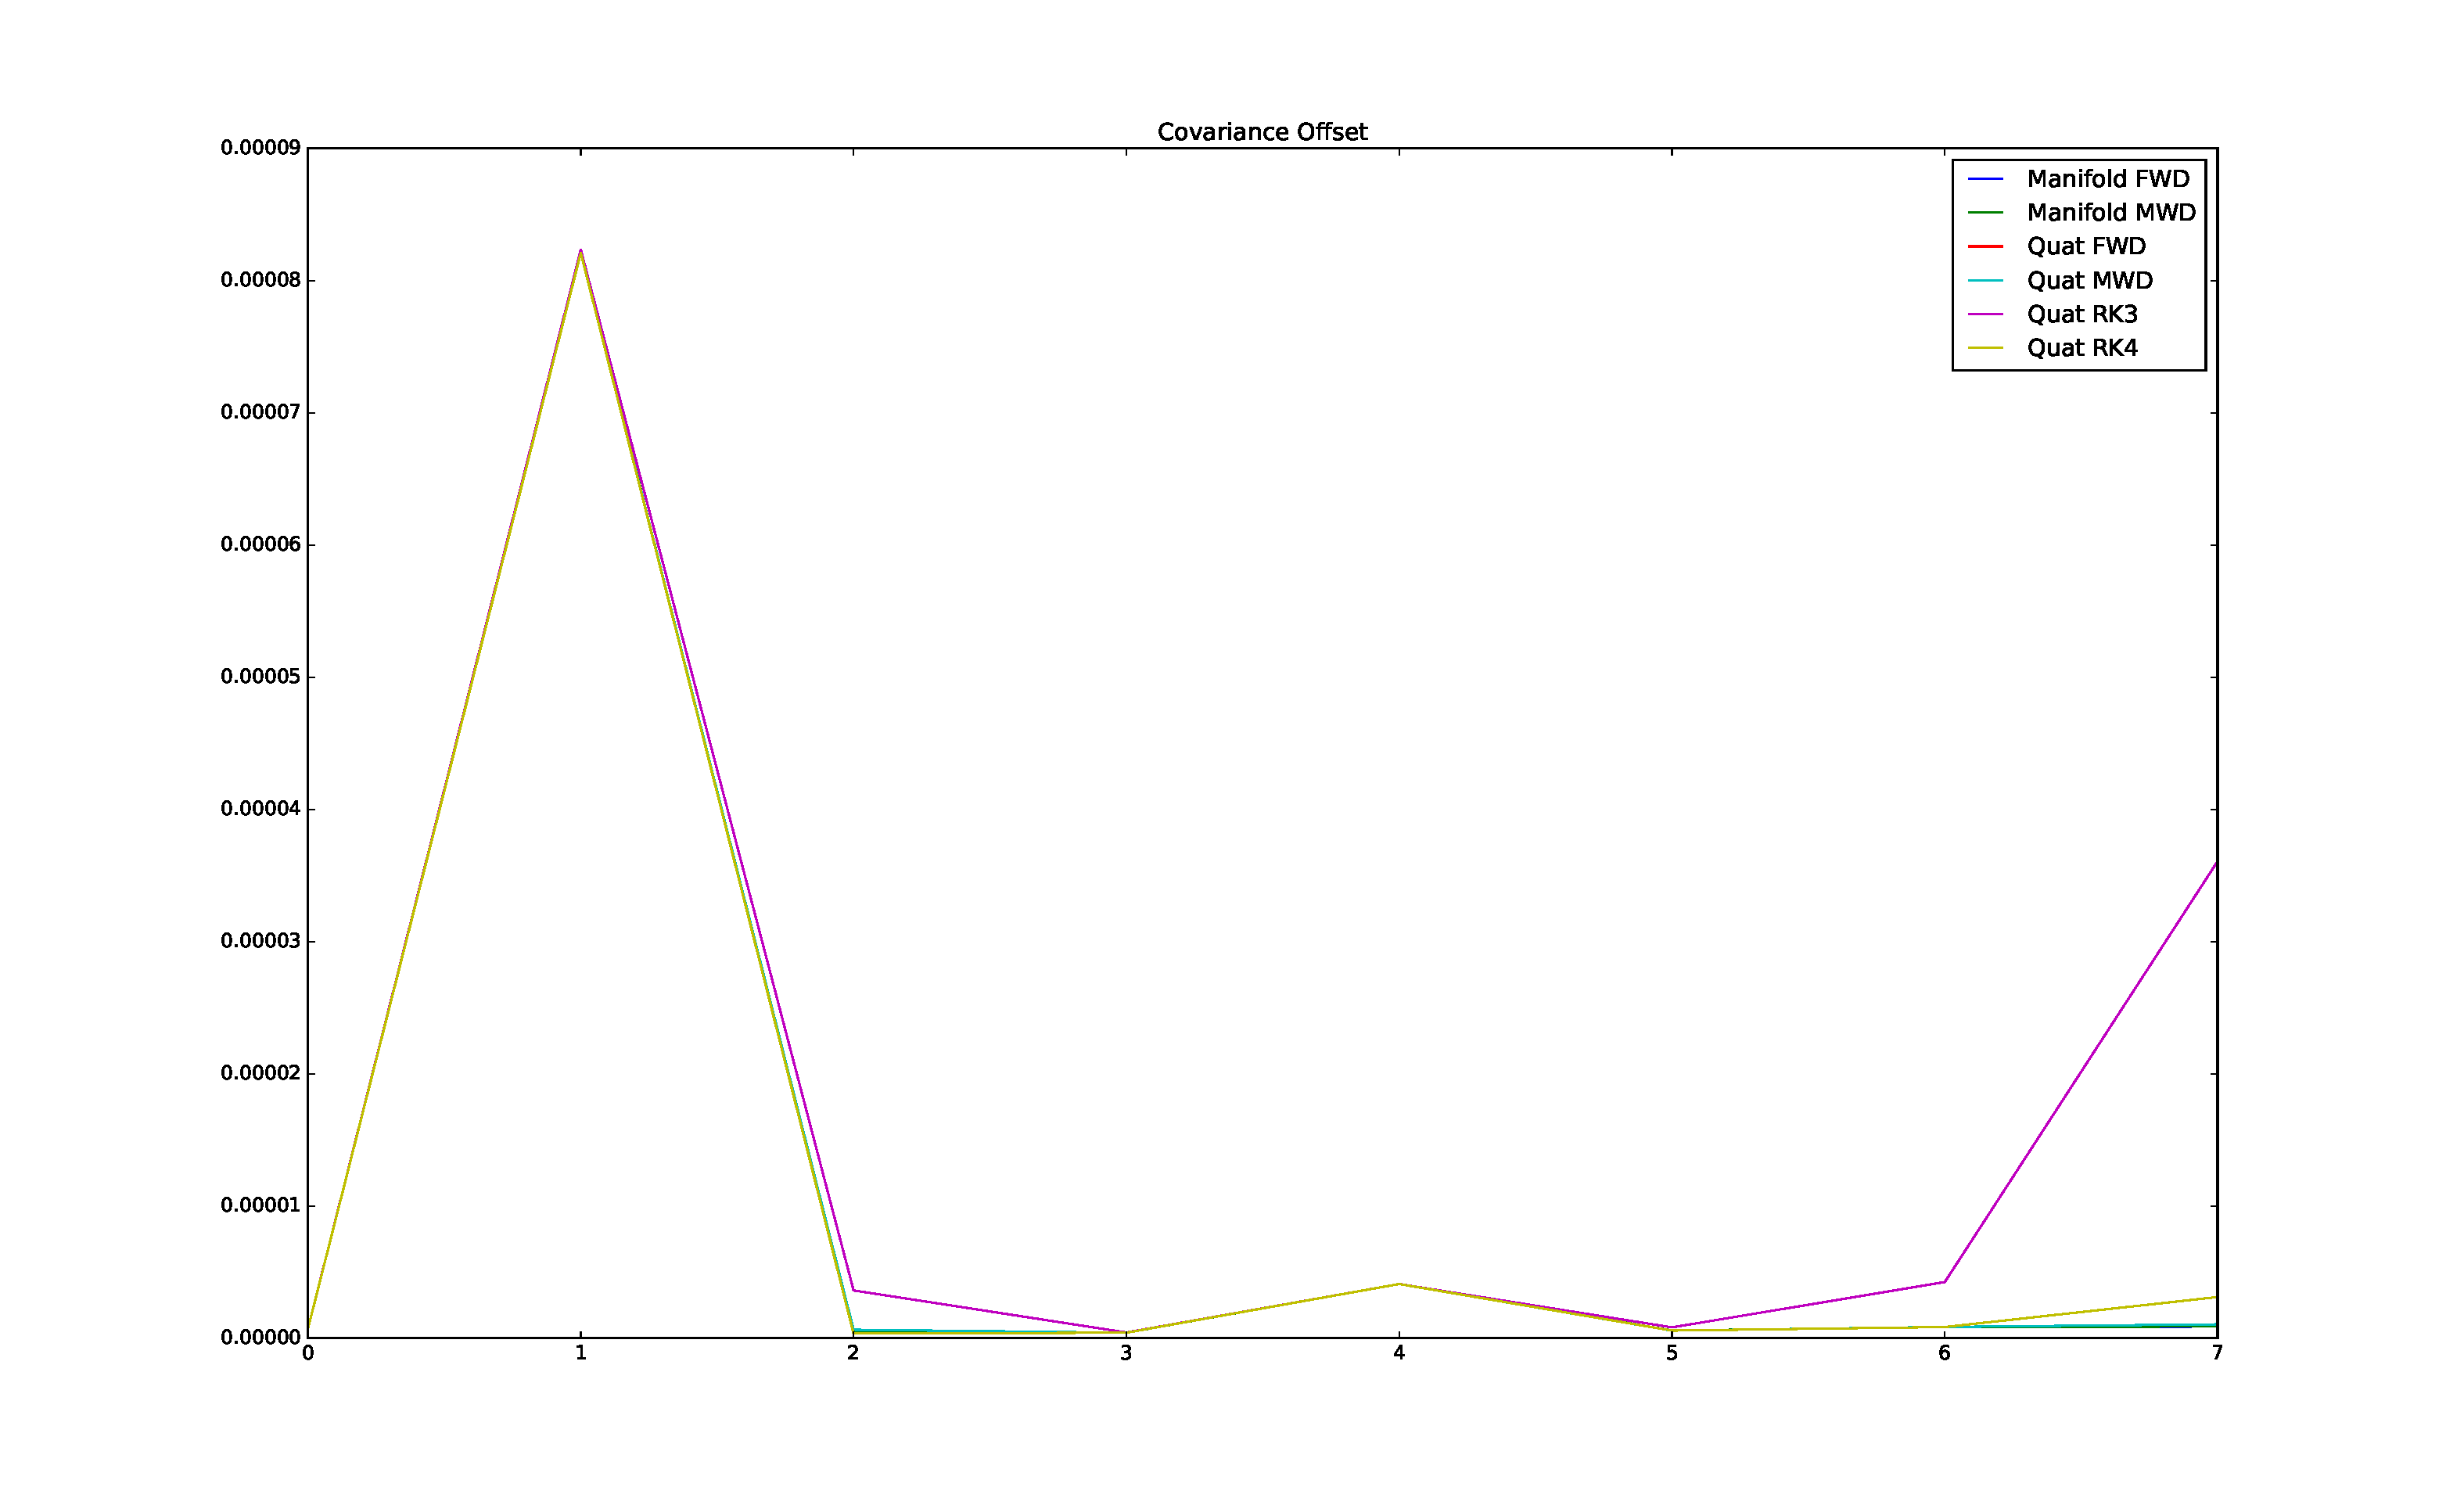
\includegraphics[width=14cm]{figures/covariance_offset_methods.pdf}
\caption{Noise propagation for different trajectories.}
\label{fig:covariance_propagation_offsets}
\end{figure}	


\begin{table}
\begin{center}
\begin{tabular}{ l | l | l | l | l | l | l}
Run & $Hz$ & Spline Order & Noise ($1e4$) & Segments & Smoothing & Rotation Multiplier \\
0 & 200 & 5 & 1.86 & 50 & $1e-6$ & 1 \\
1 & 200 & 5 & 18.6 & 50 &  $1e-6$ & 1 \\
2 & 20 & 5 & 1.86 & 50 &  $1e-6$ & 1 \\
3 & 100 & 5 & 1.86 & 50 &  $1e-6$ & 1 \\
4 & 1000 & 5 & 1.86 & 50 &  $1e-6$ & 1 \\
5 & 200 & 5 & 1.86 & 200 &  $1e-6$ & 2 \\
6 & 200 & 5 & 1.86 & 200 & $1e-6$ & 4 \\
7 & 200 & 5 & 1.86 & 200 & $1e-6$ & 10 \\
\end{tabular}
\end{center}
\caption{Parameters used to generate different trajectories for the covariance propagation evaluation.}
\label{tbl:rotation_integration_covariance_run_parameters}
\end{table}


\begin{table}
\begin{center}
\begin{tabular}{ l | l | l | l | l | l | l | l | l }
 & 0 & 1& 2 & 3 & 4 & 5 & 6 & 7 \\
0 & 7.42013e-7 & 8.21704e-5 & 4.68377e-7 & 4.20485e-7 & 4.10374e-6 & 5.86244e-7 & 8.50302e-7 & 8.86004e-7 \\
1 & 7.42001e-7 & 8.21675e-5 & 4.95865e-7 & 4.20391e-7 & 4.10374e-6 & 5.86208e-7 & 8.50439e-7 & 8.9136e-7 \\
2 & 7.41973e-7 & 8.21019e-5 & 6.472e-7 & 4.22319e-7 & 4.10381e-6 & 5.80872e-7 & 8.5574e-7 & 1.0576e-6 \\
3 & 7.41973e-7 & 8.21019e-5 & 6.472e-7 & 4.22319e-7 & 4.10381e-6 & 5.80872e-7 & 8.5574e-7 & 1.0576e-6 \\
4 & 7.42765e-7 & 8.2346e-5 & 3.61947e-6 & 4.38474e-7 & 4.10378e-6 & 8.23784e-7 & 4.25238e-6 & 3.60825e-5 \\
5 & 7.41974e-7 & 8.21021e-5 & 3.52353e-7 & 4.22279e-7 & 4.10381e-6 & 5.81326e-7 & 8.50033e-7 & 3.11836e-6
\end{tabular}
\end{center}
\caption{Covariance offset for different integration methods (rows) and trajectories (columns)}
\label{tbl:rotation_integration_covariance_values}
\end{table}

\subsection{Computational Complexity}

\begin{figure}
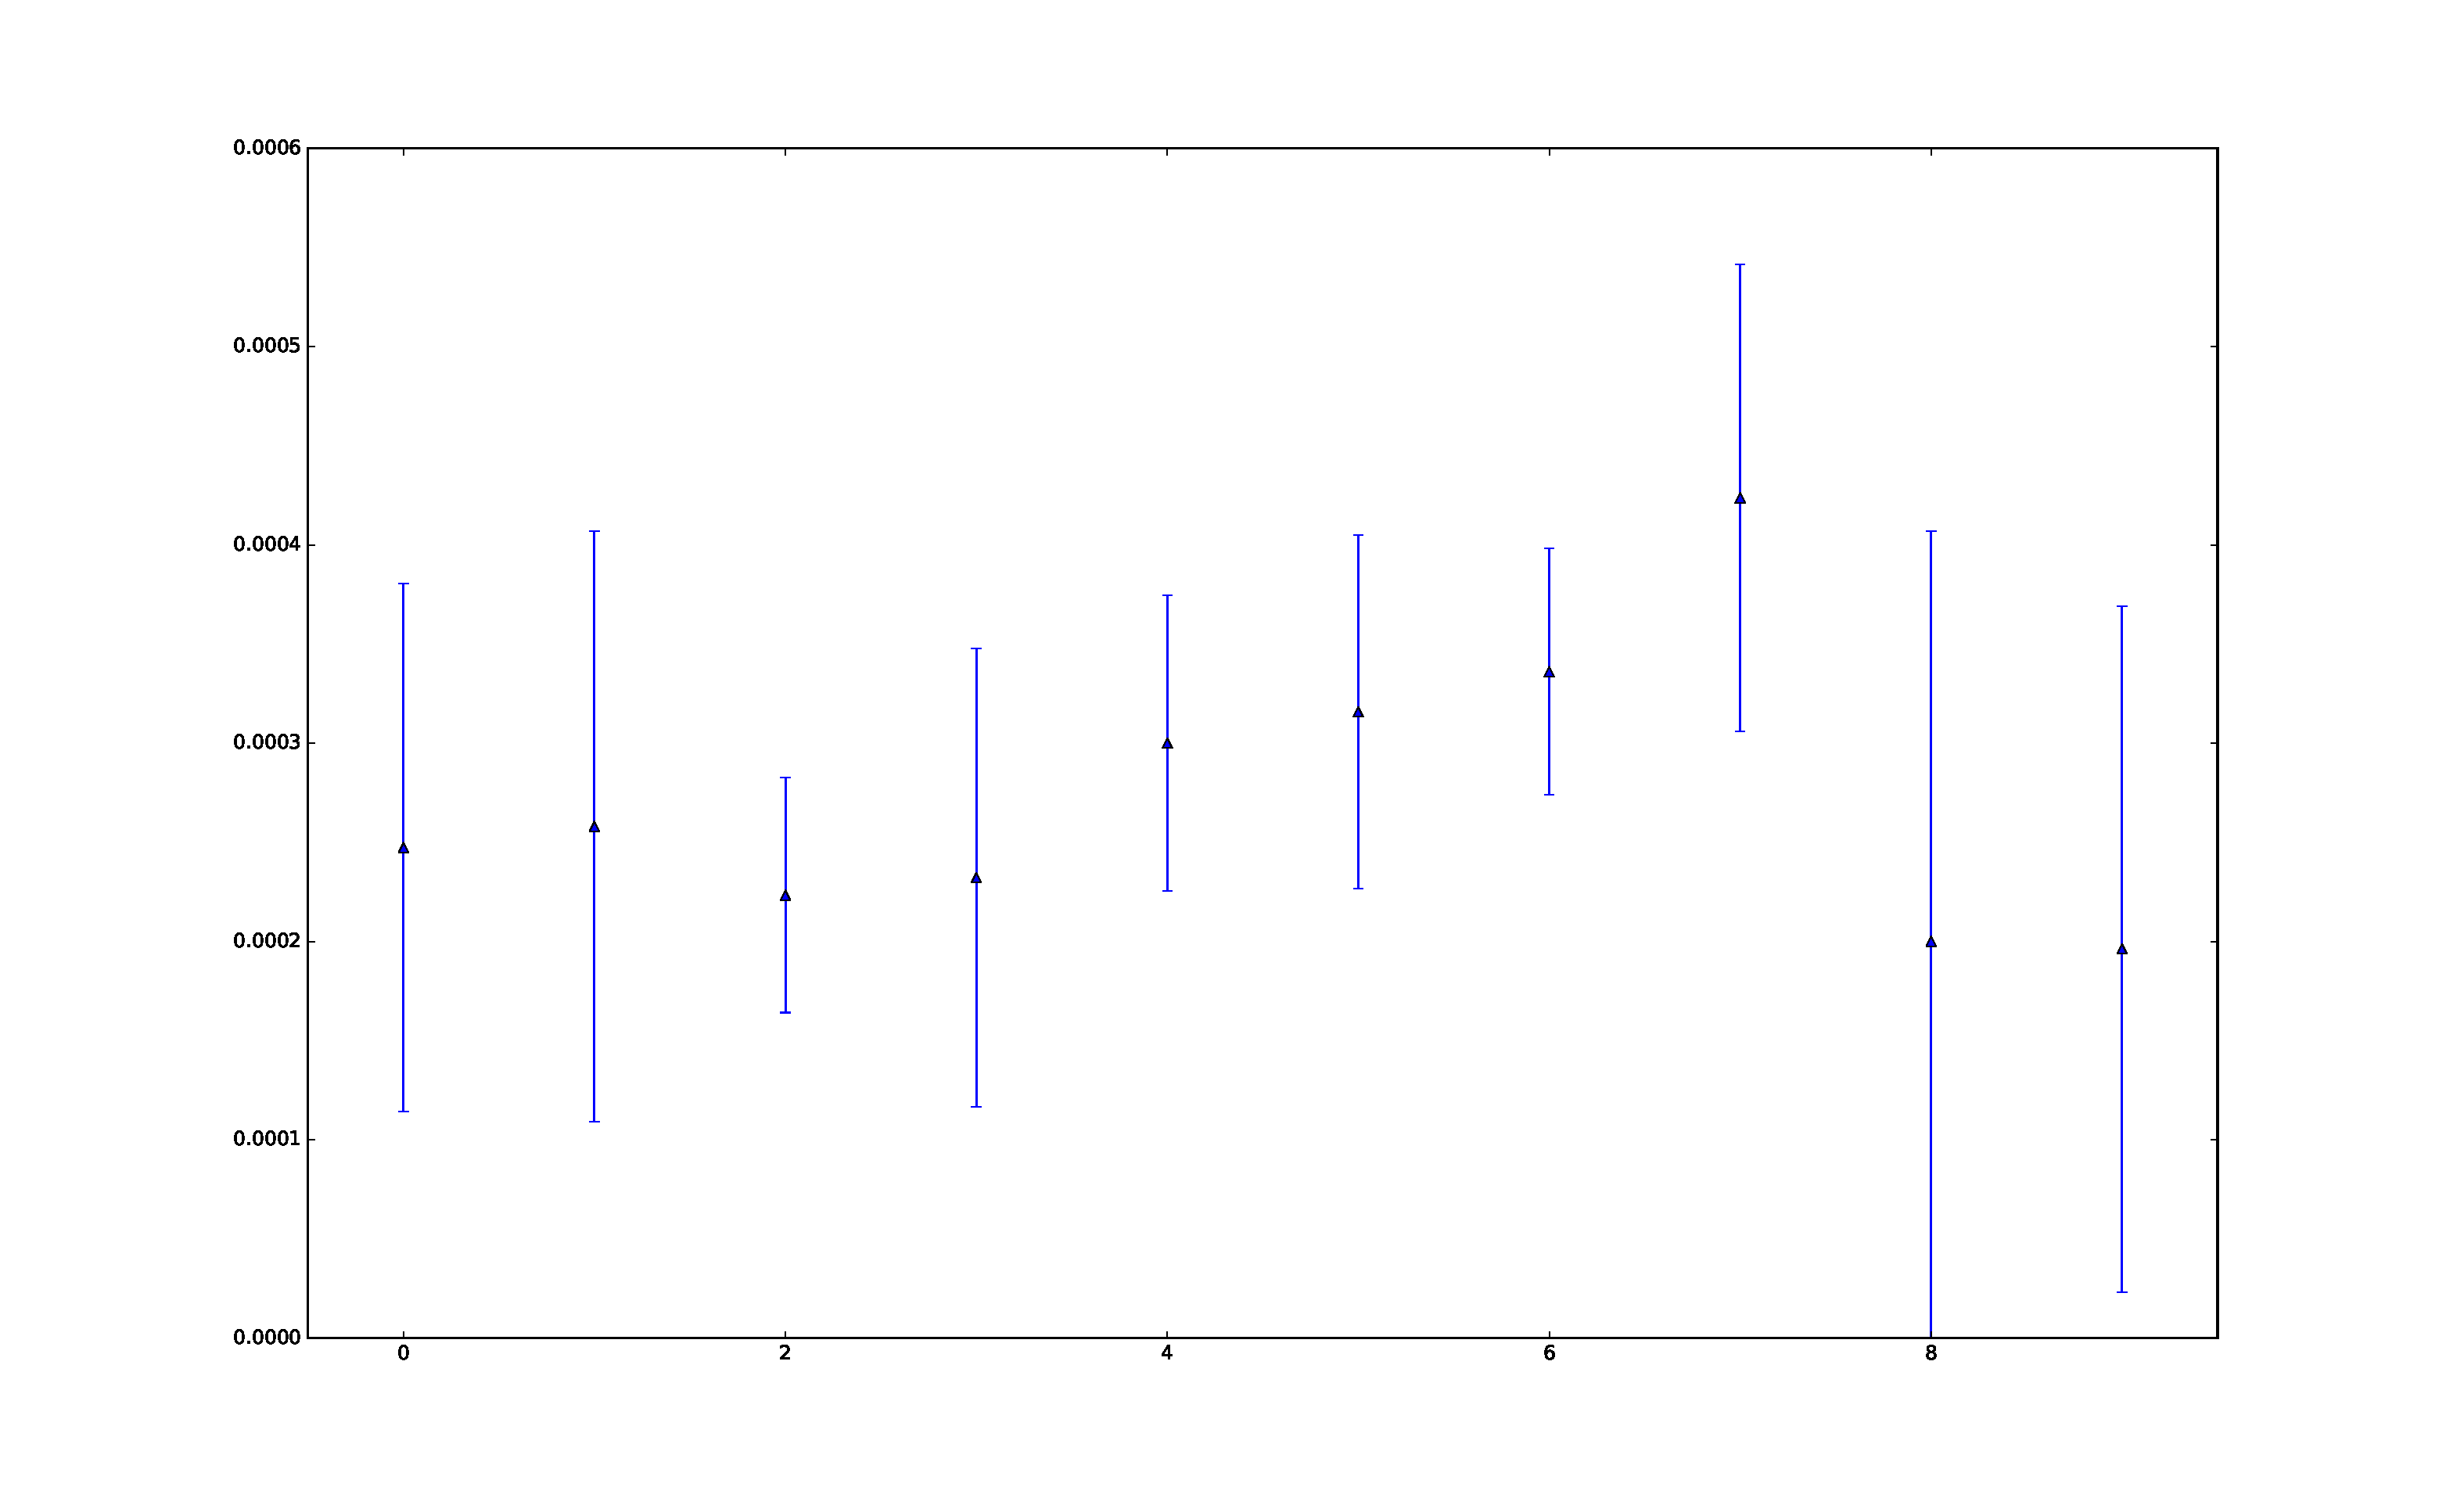
\includegraphics[width=14cm]{figures/integrator_timings.pdf}
\caption{Timings of the integrators - averages after $250'000$ steps. The indices $8$ and $9$ use the simplified On-Manifold covariance propagation.}
\label{fig:integration_timings}
\end{figure}	

The execution times of single integration steps are shown in Figure \ref{fig:integration_timings}. The times include the integration itself and the the covariance propagation step - except for the two Crouch-Grossman methods which only contain the integration and a quaternion forward covariance propagation.
As one might expect, any method that involves higher order computations and / or evaluations of exponential maps tends to be more expensive. Especially the Crouch-Grossman approaches tend to be much more expensive, even without a proper covariance propagation step. The cheapest method in terms of computational complexity and quality of the integration is the Quaternion Midward integration.

The proposed simplification of the on-manifold noise propagation slightly improves the performance and brings the on-manifold integration onto a same level with a zeroth order quaternion integration.

\section{General Integration Methods}
A thorouh introduction to integration methods with application to error state Kalman filtering is given in \cite{joan_sola}.

For a differential equation of the form:
\begin{equation}
\dot{\textbf{x}} = f(t, \textbf{x})
\end{equation}
evaluated at discrete time intervals $\textbf{x}_n$, we sample the associated values of $\dot{\mbf x}_i$.

\subsection{Zeroth Order}
Assuming that the value of $f(t)$ is piece-wise constant, and given the values $\dot{\mbf x}_i$, $\dot{\mbf x}_{i+1}$, three methods emerge immediately.

We assume that the value of $\dot{\mbf x}$ corresponds to the sample $\dot{\mbf x}_i$:
\begin{equation}
\mbf x_{i+1} = \mbf x_{i} + \Delta t \dot{\mbf x}_i,
\label{eq:first_order_forward}
\end{equation}

It is also perfectly valid, to assume that the value of $\dot{\mbf x}$ corresponds to the sample $\dot{\mbf x}_{i+1}$:
\begin{equation}
\mbf x_{i+1} = \mbf x_{i} + \Delta t \dot{\mbf x}_{i+1}.
\label{eq:first_order_backward}
\end{equation}

Both methods perform well in noise-free situations. Applying a midpoint integration is more robust to noisy values of $\dot{\mbf x}_i$ as it implements an implicit averaging filter:
\begin{equation}
\mbf x_{i+1} = \mbf x_{i} + \dfrac{1}{2}\Delta t \left( \dot{\mbf x}_{i} + \dot{\mbf x}_{i+1} \right).
\label{eq:first_order_midward}
\end{equation}


\subsection{Runge-Kutta}
\label{sec:runge-kutta}
The generalized Runge-Kutta method of $n$'th order iterates the following steps:
\begin{align}
\mbf x_{i+1} & = \mbf x_{i} + \Delta t \sum_{i = 1}^{n} b_i k^{(i)}, \\ 
\mbf k^{(i)} & = \mbf f(\mbf q^{(i)}, t_k + c_i \Delta t), \\
\mbf q^{(i)} & = \mbf q_k + \Delta t \sum_{j = 1}^{i - 1}a_{ij}\mbf k^{(i)},
\end{align}
where $a_{ij}$, $b_i$ and $c_i$ are given parameters typically represented in a Butcher table.

As the values of $f$ are typically not available explicitly but sample at discrete time-steps, $t_i$, one would linearly interpolate
the values at $t_i$ and $t_{i+1}$ to come up with an estimate at $t_i + c_i \Delta t$.

\begin{thebibliography}{}

\bibitem{joan_sola} Quaternion kinematics for the error-state KF. Joan Solà February 2, 2016, http://www.iri.upc.edu/people/jsola/JoanSola/objectes/notes/kinematics.pdf

\bibitem{andrle_crassidist} Andrle, Michael S., and John L. Crassidis. Geometric integration of quaternions. Journal of Guidance, Control, and Dynamics 36.6 (2013): 1762-1767.

\bibitem{forster}Forster, Christian, et al. On-Manifold Preintegration Theory for Fast and Accurate Visual-Inertial Navigation. arXiv preprint arXiv:1512.02363 (2015).

\bibitem{crouch_grossman} Crouch, Peter E., and R. Grossman. Numerical integration of ordinary differential equations on manifolds. Journal of Nonlinear Science 3.1 (1993): 1-33.

\bibitem{furgale} Furgale, Paul, Timothy D. Barfoot, and Gabe Sibley. Continuous-time batch estimation using temporal basis functions. Robotics and Automation (ICRA), 2012 IEEE International Conference on. IEEE, 2012.

\end{thebibliography}

\end{document}
